\documentclass[a4paper, 11pt,oneside,openany, danish]{memoir} % Starter dokumentet af klassen memoir


%%%%%%%%%%%%%%%%%%%%%%%
% PREAMBLE %			
%%%%%%%%%%%%%%%%%%%%%%%



% Papirstørrelse og margener
\usepackage[paper=a4paper, hmargin=1.1in, vmargin=1.1in]{geometry}

% Font encoding og sprog
\usepackage[T1]{fontenc}				% Output encoding
\usepackage[utf8]{inputenc}				% Input encoding
\usepackage[danish]{babel}				% Sprog (orddeling)
\renewcommand{\danishhyphenmins}{22} 	% bedre orddeling, minimum to tegn før og efter deling
\usepackage{lmodern}  					% gør underscores pænere
\usepackage{microtype} 					% laver micro ændringer i text for at udgå luft og orddeling


%% Forside text
%\usepackage{soul} % lege lege
%\sodef\an{}{0.2em}{.9em plus.6em}{1em plus.1em minus.1em}
%\newcommand\stext[1]{\an{\scshape#1}}

% Fyldetekst (Lorem ipsum)
\usepackage{blindtext}

% Til kodeeksempler
\usepackage{listings}

\lstdefinestyle{customc}{
	belowcaptionskip=1\baselineskip,
	breaklines=true,
	frame=L,
	xleftmargin=\parindent,
	language=C,
	showstringspaces=false,
	basicstyle=\footnotesize\ttfamily,
	keywordstyle=\bfseries\color{green!40!black},
	commentstyle=\itshape\color{purple!40!black},
	identifierstyle=\color{blue},
	stringstyle=\color{orange},
}

\lstdefinestyle{customasm}{
	belowcaptionskip=1\baselineskip,
	frame=L,
	xleftmargin=\parindent,
	language=[x86masm]Assembler,
	basicstyle=\footnotesize\ttfamily,
	commentstyle=\itshape\color{purple!40!black},
}

\lstset{escapechar=@,style=customc}

% Tabeller
\usepackage{booktabs}
\usepackage{threeparttable}
\usepackage[tableposition=top]{caption}
\usepackage{tabularx}
\usepackage{multirow}					% For at lave pæne tabeller
\usepackage{hhline}						% For at lave endnu pænere tabller
\newcolumntype{C}{>{\let\newline\\\arraybackslash\hspace{0pt}}X}
\usepackage{float}
%matematik
\usepackage{amsmath,amssymb,mathtools,bm}
\newcommand{\tsub}[1]{_{\textup{#1}}}
\def\doubleunderline#1{\underline{\underline{#1}}}
\usepackage[separate-uncertainty = true,multi-part-units=single]{siunitx}
\usepackage{longtable}

% XColor: Farver
\usepackage[svgnames,dvipsnames,x11names]{xcolor}

% Figurer og floats
\usepackage[]{graphicx}
\graphicspath{{figurer/}}
\usepackage{placeins}
\usepackage{float}			% Muliggoer eksakt placering af floats, f.eks. \begin{figure}[H]

%%% Tegning af kasser
%\usepackage{calc,graphicx,color}
%\definecolor{mygreen}{rgb}{0,0.6,0}
%\definecolor{mygray}{rgb}{0.5,0.5,0.5}

% Biblatex til referencer
\usepackage[backend=bibtex]{biblatex}
\addbibresource{bibfil.bib}





% Hyper ref
\usepackage[ unicode=true, colorlinks=false, linktocpage=true, 
pdfborder={0 0 0}, pdfstartpage=1, pdfstartview=FitV, breaklinks=true,
pdfpagemode=UseNone, pageanchor=true, pdfpagemode=UseOutlines,
plainpages=false, bookmarksnumbered, bookmarksopen=true,
bookmarksopenlevel=1, hypertexnames=true, pdfhighlight=/O, urlcolor=Black,
linkcolor=Black, citecolor=Black]{hyperref}

% Clever ref
\usepackage{cleveref}



\settocdepth{subsection}
\setsecnumdepth{subsection}

% Sidetal
% Sidetal
\let\footruleskip\undefined
\usepackage{fancyhdr}
\usepackage{lastpage}
\pagestyle{fancy} 
\fancyhf{} 

\fancyhead[R]{\leftmark}
\fancyfoot[R]{\thepage \hspace{0.008in} af \pageref{LastPage}}

\fancypagestyle{}{
	\renewcommand{\headrulewidth}{0pt}
	\fancyhf{}
	\fancyfoot[R]{\thepage \hspace{0.008in} af \pageref{LastPage}}%
	
}

% Starten på dokumentet
\begin{document}


%%%%%%%%%%%%%%%%%%%%%%%
		       % FORSIDEN %			
%%%%%%%%%%%%%%%%%%%%%%%
% !TEX root = ../prj4projektdokumentation.tex
% SKAL STÅ I TOPPEN AF ALLE FILER FOR AT MASTER-filen KOMPILERES 
\thispagestyle{empty}
{\centering
	{\scshape\LARGE Aarhus Universitet \par}
	\vspace{1cm}
	{\scshape\Large 4. semesterprojekt gruppe 1\par}
	{\scshape\Large Projektdokumentation\par}
	\vspace{1.5cm}
	{\huge\bfseries Spændingsregulator\par}
	\vspace{2cm}
	{\Large
		201509249 - Caroline Møller Sørensen\\
		201611140 - Sophia Amailie Mortensen\\
		201505195 - Dennis Slot Larsen \\
		201505115 - Laurids Givskov Jørgensen\\
		201508333 - Søren Jensen\\
		13114 - Jeppe Hansen\\  }
	\vfill
	Vejleder\par
	Emir Pasic
	
	\vfill
	
	{\large \today\par}
	\par}





%%%%%%%%%%%%%%%%%%%%%%%

             % RESUME & ABSTRACT %			
             
%%%%%%%%%%%%%%%%%%%%%%%            
\section*{Resume}
% !TEX root = ../prj4projektrapport.tex
% SKAL STÅ I TOPPEN AF ALLE FILER FOR AT MASTER-filen KOMPILERES 

Denne rapport beskriver et 4. semester projekt ved Ingeniørhøjskolen Aarhus Universitet på studieretningen Elektrisk Energiteknologi. Problemstillingen, der arbejdes med, er at udvikle et system, som kan sikre et stabilt spændingsniveau på en distributionslinje med varierende belastning.

Rapporten beskriver en prototype på en spændingsregulator, som kan installeres på en eksisterende distributionslinje. Prototypen indeholder en simulering af en distributionslinje, hvorpå spændingsregulatorens funktionalitet demonstreres. Reguleringen af spændingen foretages med en trintransformer, som skifter trin på baggrund af data fra måleenheder placeret centralt og decentralt på distributionslinjen.

Projektet indeholder programmering af måleenheder på PSoC, styring af trintransformeren på en Siemens PLC og TCP-kommunikation. 
\section*{Abstract}
% !TEX root = ../prj4projektrapport.tex
% SKAL STÅ I TOPPEN AF ALLE FILER FOR AT MASTER-filen KOMPILERES 

This report describes a fourth semester project at Aarhus School of Engineering in the field of Electical Engineering. The thesis is devoted to the development of a system that ensure a stable voltage level on a distribution line with varying load.

The report describes a prototype of a voltage regulator, which can be installed on an existing distribution line. The prototype contains a simulation of a distribution line, on which the functionality of the voltage regulator is demonstrated. The voltage regulation is performed with a step transformer that changes step based on data from measurement devices placed centrally and decentrally on the distribution line. 

The project includes programming of measurement devices on PSOC, controlling/regulation of the step transformer on a Siemens PLC and TCP-communication.


\pagebreak

%%%%%%%%%%%%%%%%%%%%%%%


%%%%%%%%%%%%%%%%%%%%%%%
         % INDHOLDSFORTEGNELSE %			
%%%%%%%%%%%%%%%%%%%%%%%
\frontmatter
\tableofcontents

%%%%%%%%%%%%%%%%%%%%%%%
                        % KAPITLER %			
%%%%%%%%%%%%%%%%%%%%%%%                        
\mainmatter
\chapter{Forord}  
% !TEX root =../prj4projektrapport.tex



\textbf{Praktisk information:} I dette projekt deltog seks ingeniørstuderende fra Ingeniørhøjskolen Aarhus Universitet. De studerende er på 4. semester på studieretningen Elektrisk Energiteknologi. Projektgruppens vejleder er Emir Pasic, der løbende har vejledt gruppen. Semesterprojektets afleveringsdato er 29/5-2017 og bedømmelsesdato er 28/6-2017. \\
\textbf{Læsevejledning:} Henvisninger til projektdokumentationen er lavet med fodnoter, der angiver kapitelnummer og navn på det afsnit, der henvises til. Bilagshenvisninger er lavet med mappenavn og bilagsnummer. \\
\textbf{Tak til:} Der skal tilskrives en tak til Michael Rangård, Specialist Planlægning, og Poul Bagger Thomsen, Afdelingsleder Anlæg 20/0,4kV, fra Eniig for hjælp med data og besøg på transformerstation.
                     
\chapter{Indledning}
% !TEX root =../prj4projektrapport.tex

Formålet med dette projekt er at løse følgende problemformulering; \textit{Når belastningerne i et distributionssystem ændres, vil spændingsniveauet variere. Det er vigtigt, at spændingsniveauet holdes stabilt. Hvordan sikres dette?}
Udgangspunktet for problemstillingen er det lovmæssige krav, der siger, at spændingsforsyningen hos danske forbrugere altid skal ligge på 230V $\pm$10$\%$ \cite{Sikkerhedsstyrelsen}. Det ønskes at undersøge udfordringerne ved dette samt at komme med et bud på, hvordan denne problemstilling løses bedst muligt, både som elnettet ser ud i dag, men også i fremtiden. 

For at kunne arbejde med problemformuleringen og undersøge dens aktualitet, valgte projektgruppen at tage kontakt til energiselskabet Eniig. Det viste sig, at der på nuværende tidspunkt ikke foretages regulering på lavspændingsnettet, men i stedet på 60/10 kV transformere. Projektgruppen fandt det derfor interessant at undersøge mulighederne for regulering på lavspændingsnettet og eventuelle fordele og fremtidsaspekter ved dette.

I dette projekt vil fokus derfor være på den del af nettet, der går fra distributionstransformer og ud til forbrugere. For at sikre et stabilt spændingsniveau ønskes det at kunne overvåge tilstanden på distributionslinjen, ikke kun ved transformeren, men også ved hver enkelt forbruger. Det samlede system, der fremstilles i projektet betegnes som Spændingsregulator. Med denne ønskes det at lave et proof of concept i forhold til problemformuleringen. På grund af tilgængelighed af komponenter og udstyr vil prototypen for Spændingsregulator blive skaleret ned. 

For at belyse problemstillingen vil der i dette projekt blive lavet en simulering af en distributionslinje samt belastninger, der skal simulere forbrugere på linjen. Projektet vil desuden bestå af en trintransformer, der giver mulighed for at variere spændingsniveauet til linjen og forbrugerne på sekundærsiden af transformeren.

Til justering af spændingsniveauet, er det nødvendigt at kende til de aktuelle værdier for spændingen både centralt ved trintransformeren og decentralt ved forbrugerne. Af denne grund implementeres enheder til måling af spændingen. Det ønskes desuden at kende til systemets power factor, og derfor skal strømmen også måles. Et eventuelt indhold af harmoniske kan føre til unødig belastning og opvarmning af transformere, og det er derfor fornuftigt at kende til indholdet af harmoniske, og denne parameter skal også måles.
For at kunne holde et ønsket spændingsniveau vil der i projektet implementeres en enhed til regulering af trin på transformeren.

\begin{figure}[H]
	\centering
	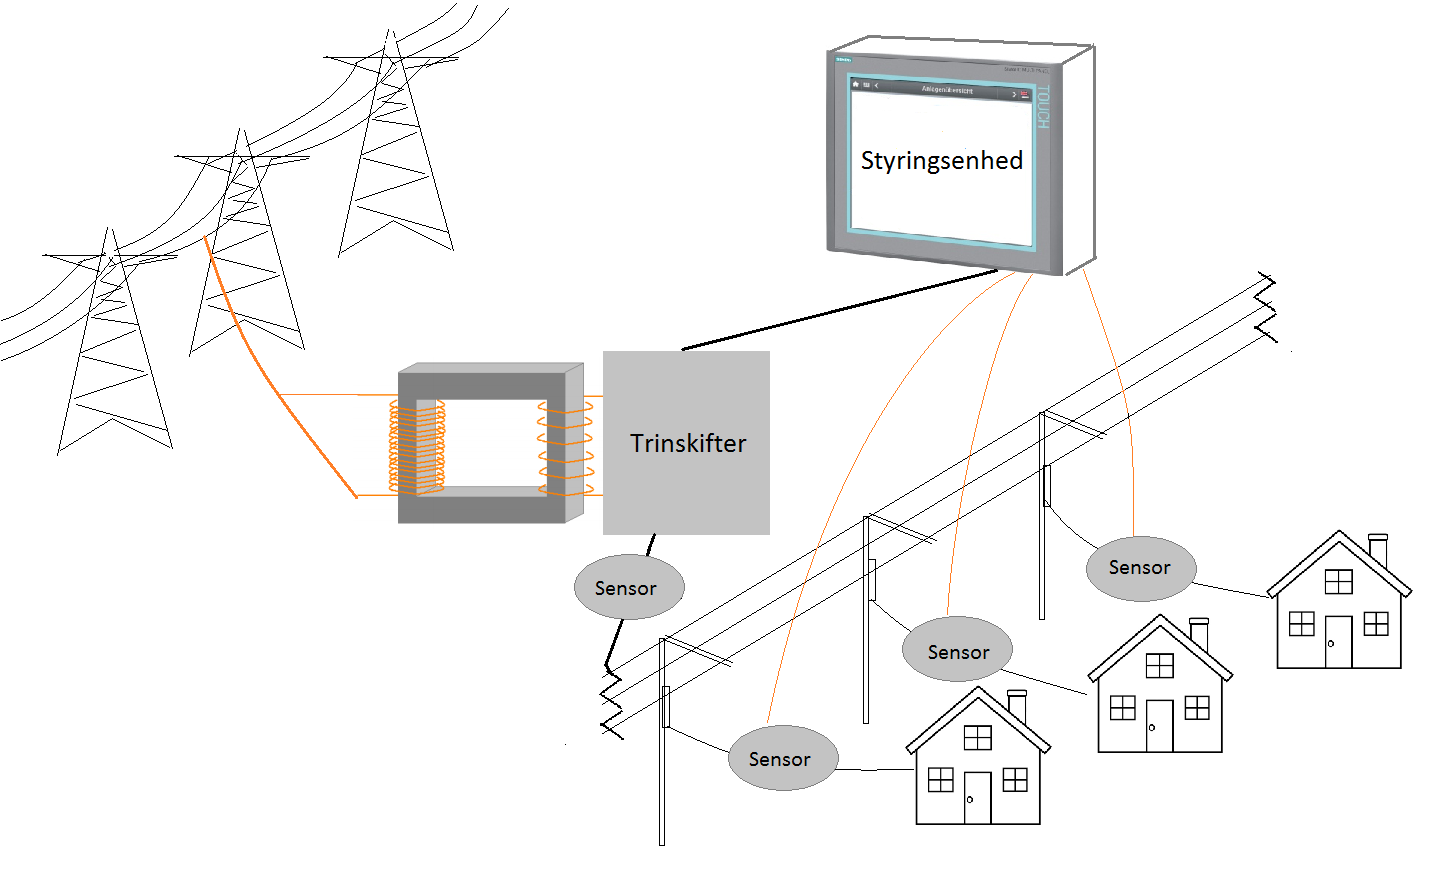
\includegraphics[width=1\textwidth]{figure/RigtBillede}
	\caption{Visuel fremstilling af Spændingsregulator}
	\label{fig:Rigtbillede}
\end{figure}

På figur \ref{fig:Rigtbillede} ses en illustration, der giver oveblik over Spændingsregulatoren. Billedet viser trintransformeren, der forsyner distributionslinjen, sensorer, der måler aktuelle værdier på linjen og en styringsenhed, der regulerer trintransformeren på baggrund af disse værdier. 
\chapter{Kravspecifikation}
% !TEX root = ../prj4projektrapport.tex
% SKAL STÅ I TOPPEN AF ALLE FILER FOR AT MASTER-filen KOMPILERES 

Dette kapitel indeholder en overordnet beskrivelse af systemet, samt en gennemgang af de funktionelle og ikke funktionelle krav der stilles til systemet. 

\section{Systembeskrivelse}
Spændingsregulatoren skal være i stand til at analysere forholdene på distributionslinjen. Derfor udvikles en måleenhed, som kan placeres decentralt, ved hver forbruger, og centralt ved spændingsregulatoren. Måleenhederne skal sende værdier for spænding, strøm, powerfactor og indhold af harmoniske til et system, som regulerer spændingen på baggrund af disse målinger. 

Spændingsreguleringen laves med en trintransformer, hvor der med en styringsenhed kan skiftes mellem trinene. Styringsenheden kan automatisk regulere spændingen jf. data fra måleenhederne, eller den kan styres manuelt på en grafisk brugergrænseflade. 

Systemet der er udviklet i dette projekt er proof of concept, så spændingsniveauet er skalleret ned.  Der er designet et simuleringskredsløb i form af en distributionslinje og en række forbrugere, for at vise funktionaliteten af Spændingsregulatoren. Forbrugerene  kan kobles til/fra nettet, for at generere et spændingsfald der giver anledning til en regulering af trintransformeren. 


% !TEX root = ../../prj4projektdokumentation.tex
% SKAL STÅ I TOPPEN AF ALLE FILER FOR AT MASTER-filen KOMPILERES 

\section{Funktionelle krav}
I dette afsnit beskrives de funktionelle krav for systemet. De dele, hvor en bruger interager med systemet er beskrevet med usecase diagrammer. Den automatiske del er beskrevet og vist vha. et STM diagram.

\subsection{Beskrivelse af automatisk mode}
\label{Afsnit: Automatisk mode}

Når spændingsregulatoren er i automatisk mode, kontrolleres spænding ved forbrugerne. Hvis den spænding er for høj eller lav iht. de 4V skiftes der et trin op eller et trin ned.  
\begin{figure}[htbp] % (alternativt [H])
	\centering
	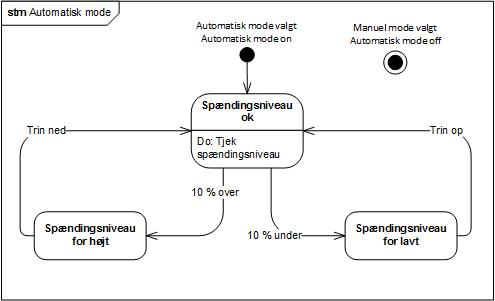
\includegraphics[width=0.8\textwidth]{Figure/STM}
	\caption{Beskrivelse af automatisk mode}
	\label{fig:automode}
\end{figure}

\subsection{Usecase Diagram}

\begin{figure}[H] % (alternativt [H])
	\centering
	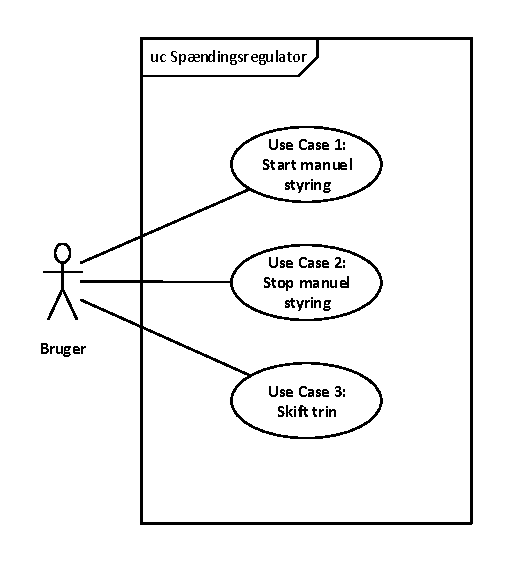
\includegraphics[width=0.5\textwidth]{Figure/UsecaseDiagram}
	\caption{Usecase Diagram}
	\label{fig:UsecaseDiagram}
\end{figure}
Systemet indholder tre usecases, der alle er initieret af brugeren. Den automatiske del af systemet er beskrevet i afsnit \ref{Afsnit: Automatisk mode}.

\subsection{Aktør Beskrivelse}
\textbf{Brugeren} er den primær aktør. En sikkerhedsgodkendt operatør der kan betjene systemet.

\subsection{Usecase 1 - Start manuel styring}
\begin{table}[H]
	\centering
	
	\begin{threeparttable}
		\begin{tabularx}{\linewidth}{ l X }
			\toprule
			\bfseries{Navn:}				& UC1 - Start manuel styring  \\
			\midrule
			\bfseries{Mål:} 				& At sætte systemet i manuel mode \\
			\midrule
			\bfseries{Initiering:} 			& Initieres af brugeren. \\
			\midrule
			\bfseries{Aktører:} 			& Brugeren (Primær) \\
			\midrule
			\bfseries{Samtidige forekomster:} & 1 \\
			\midrule
			\bfseries{Forudsætninger:} 		& At systemet er funktionelt og i automatisk mode\\
			\midrule
			\bfseries{Resultat:} 			& Systemet er i manuel mode \\
			\midrule
			\bfseries{Hovedscenariet:} 	& \\
			
			
			1 	& Brugeren trykker Manuel styring på skærmen.\\
			2	& Systemet skifter til Manuel mode. \\
			3 	& Systemet aktivere manuel skærm. 	\\
			
			\bottomrule
			
		\end{tabularx}
	\end{threeparttable}
	\caption{Fully dressed use case for UC1 - Start manuel styring}
	\label{table:UC1}
\end{table}

\subsection{Usecase 2 - Stop manuel styring}

\begin{table}[H]
	\centering
	
	\begin{threeparttable}
		\begin{tabularx}{\linewidth}{ l X }
			\toprule
			\bfseries{Navn:}				& UC2 - Stop manuel styring  \\
			\midrule
			\bfseries{Mål:} 				& At sætte systemet i automatisk mode \\
			\midrule
			\bfseries{Initiering:} 			& Initieres af brugeren. \\
			\midrule
			\bfseries{Aktører:} 			& Brugeren (Primær) \\
			\midrule
			\bfseries{Samtidige forekomster:} & 1 \\
			\midrule
			\bfseries{Forudsætninger:} 		& At systemet er funktionelt og i manuel mode\\
			\midrule
			\bfseries{Resultat:} 			& Systemet er i automatisk mode \\
			\midrule
			\bfseries{Hovedscenariet:} 	& \\
			
			
			1 	& Brugeren trykker Automatisk styring på skærmen.\\
			2 	& Systemet skifter til Automatisk mode.\\
			3 	& Systemet aktivere automatisk skærm. 	\\		
				
			
			\bottomrule
			
		\end{tabularx}
	\end{threeparttable}
	\caption{Fully dressed use case for UC2 - Stop manuel styring}
	\label{table:UC2}
\end{table}

\subsection{Usecase 3a - Skift trin}

\begin{table}[H]
	\centering
	
	\begin{threeparttable}
		\begin{tabularx}{\linewidth}{ l X }
			\toprule
			\bfseries{Navn:}				& UC3a - Skift trin op  \\
			\midrule
			\bfseries{Mål:} 				& At skifte et trin op på transformeren \\
			\midrule
			\bfseries{Initiering:} 			& Initieres af brugeren. \\
			\midrule
			\bfseries{Aktører:} 			& Brugeren (Primær) \\
			\midrule
			\bfseries{Samtidige forekomster:} & 1 \\
			\midrule
			\bfseries{Forudsætninger:} 		& At systemet er funktionelt og i manuel mode\\
			\midrule
			\bfseries{Resultat:} 			& Transformerens trin er skiftet et trin op \\
			\midrule
			\bfseries{Hovedscenariet:} 	& \\
			
			
			1 	& Brugeren vælger Trin Op på skærmen.\\
			2 	& Systemet skifter et trin op på transformeren.\\
			3 	& Aktuelt trin vises på skærmen.\\
			4 	& Måleværdier opdateres på skærmen.\\		
			
			\bottomrule
			
		\end{tabularx}
	\end{threeparttable}
	\caption{Fully dressed use case for UC3 - Skift trin}
	\label{table:UC3}
\end{table}

\subsection{Usecase 3b - Skift trin}

\begin{table}[H]
	\centering
	
	\begin{threeparttable}
		\begin{tabularx}{\linewidth}{ l X }
			\toprule
			\bfseries{Navn:}				& UC3b - Skift trin ned  \\
			\midrule
			\bfseries{Mål:} 				& At skifte et trin ned på transformeren \\
			\midrule
			\bfseries{Initiering:} 			& Initieres af brugeren. \\
			\midrule
			\bfseries{Aktører:} 			& Brugeren (Primær) \\
			\midrule
			\bfseries{Samtidige forekomster:} & 1 \\
			\midrule
			\bfseries{Forudsætninger:} 		& At systemet er funktionelt og i manuel mode\\
			\midrule
			\bfseries{Resultat:} 			& Transformerens trin er skiftet et trin ned \\
			\midrule
			\bfseries{Hovedscenariet:} 	& \\
			
			
			1 	& Brugeren vælger Trin Ned på skærmen.\\
			2 	& Systemet skifter et trin ned på transformeren.\\
			3 	& Aktuelt trin vises på skærmen.\\
			4 	& Måleværdier opdateres på skærmen.\\			
			
			\bottomrule
			
		\end{tabularx}
	\end{threeparttable}
	\caption{Fully dressed use case for UC3 - Skift trin}
	\label{table:UC3}
\end{table}



% !TEX root = ../prj4projektrapport.tex
% SKAL STÅ I TOPPEN AF ALLE FILER FOR AT MASTER-filen KOMPILERES 

\section{Ikke Funktionelle Krav}

% !TEX root = ../prj4projektrapport.tex
% SKAL STÅ I TOPPEN AF ALLE FILER FOR AT MASTER-filen KOMPILERES 


\section{Afgrænsning}
Afgrænsning af projektet er lavet som MoSCoW. Der beskrives hvad, der skal med i projektet, for at det fungere og hvad der ikke er så vigtigt. Der er i projektet ikke taget højde for optimering, men kun at der skal være et færdigt funktionelt produkt.
\subsubsection{MoSCoW}

\begin{itemize}
	\item{Systemet \textbf{skal} bestå af en trinskifter 24/0-8V}
	\item{Systemet \textbf{skal} måle spænding, strøm, power factor og harmoniske centralt og decentralt}
	\item{Systemet \textbf{skal} vise data på en skærm}
	\item{Systemet \textbf{skal} simulere en distributionslinje og flere forbrugere}
	\item{Systemet \textbf{skal} kunne reguleres manuelt}
	\item{Systemet \textbf{burde} kunne reguleres automatisk}
	\item{Systemet \textbf{kunne} have en log}
	\item{Distributionslinjen \textbf{kunne} indeholde en decentral producent}
	\item{Systemet \textbf{vil ikke} fjerne harmoniske} 
\end{itemize}	
\chapter{Arkitektur}
% !TEX root =../prj4projektrapport.tex

Formålet med dette projekt er at løse følgende problemformulering; \textit{Når belastningerne i et distributionssystem ændres, vil spændingsniveauet variere. Det er vigtigt, at spændingsniveauet holdes stabilt. Hvordan sikres dette?}
Udgangspunktet for problemstillingen er det lovmæssige krav, der siger, at spændingsforsyningen hos danske forbrugere altid skal ligge på 230V $\pm$10$\%$ \cite{Sikkerhedsstyrelsen}. Det ønskes at undersøge udfordringerne ved dette samt at komme med et bud på, hvordan denne problemstilling løses bedst muligt, både som elnettet ser ud i dag, men også i fremtiden. 

For at kunne arbejde med problemformuleringen og undersøge dens aktualitet, valgte projektgruppen at tage kontakt til energiselskabet Eniig. Det viste sig, at der på nuværende tidspunkt ikke foretages regulering på lavspændingsnettet, men i stedet på 60/10 kV transformere. Projektgruppen fandt det derfor interessant at undersøge mulighederne for regulering på lavspændingsnettet og eventuelle fordele og fremtidsaspekter ved dette.

I dette projekt vil fokus derfor være på den del af nettet, der går fra distributionstransformer og ud til forbrugere. For at sikre et stabilt spændingsniveau ønskes det at kunne overvåge tilstanden på distributionslinjen, ikke kun ved transformeren, men også ved hver enkelt forbruger. Det samlede system, der fremstilles i projektet betegnes som Spændingsregulator. Med denne ønskes det at lave et proof of concept i forhold til problemformuleringen. På grund af tilgængelighed af komponenter og udstyr vil prototypen for Spændingsregulator blive skaleret ned. 

For at belyse problemstillingen vil der i dette projekt blive lavet en simulering af en distributionslinje samt belastninger, der skal simulere forbrugere på linjen. Projektet vil desuden bestå af en trintransformer, der giver mulighed for at variere spændingsniveauet til linjen og forbrugerne på sekundærsiden af transformeren.

Til justering af spændingsniveauet, er det nødvendigt at kende til de aktuelle værdier for spændingen både centralt ved trintransformeren og decentralt ved forbrugerne. Af denne grund implementeres enheder til måling af spændingen. Det ønskes desuden at kende til systemets power factor, og derfor skal strømmen også måles. Et eventuelt indhold af harmoniske kan føre til unødig belastning og opvarmning af transformere, og det er derfor fornuftigt at kende til indholdet af harmoniske, og denne parameter skal også måles.
For at kunne holde et ønsket spændingsniveau vil der i projektet implementeres en enhed til regulering af trin på transformeren.

\begin{figure}[H]
	\centering
	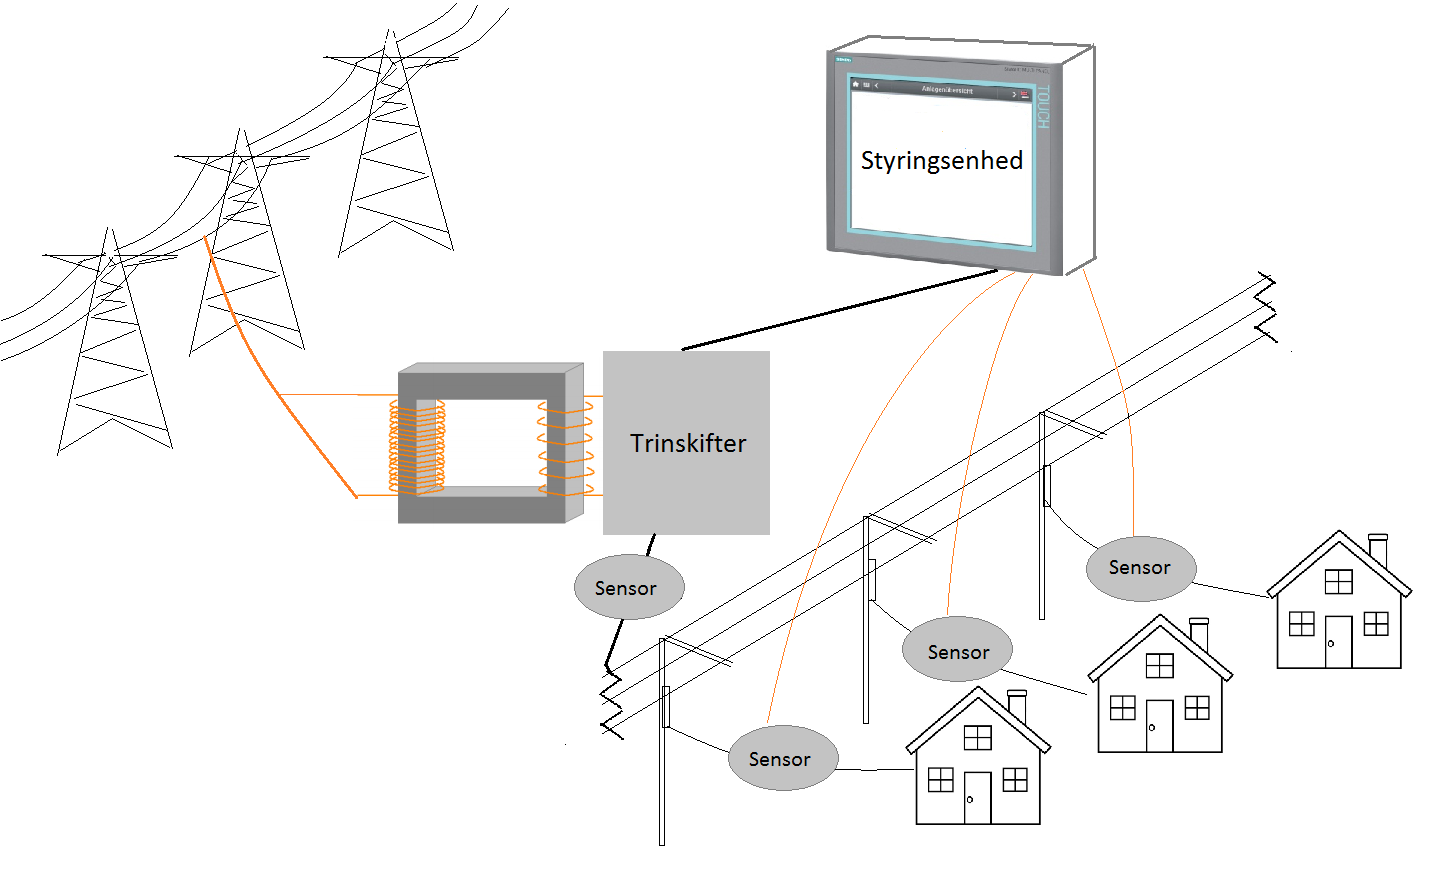
\includegraphics[width=1\textwidth]{figure/RigtBillede}
	\caption{Visuel fremstilling af Spændingsregulator}
	\label{fig:Rigtbillede}
\end{figure}

På figur \ref{fig:Rigtbillede} ses en illustration, der giver oveblik over Spændingsregulatoren. Billedet viser trintransformeren, der forsyner distributionslinjen, sensorer, der måler aktuelle værdier på linjen og en styringsenhed, der regulerer trintransformeren på baggrund af disse værdier. 
% !TEX root = ../../prj4projektdokumentation.tex
% SKAL STÅ I TOPPEN AF ALLE FILER FOR AT MASTER-filen KOMPILERES 

\section{Blok definitionsdiagram}
Et BDD for spændingsregulator ses på figur \ref{fig:BDDSpaendingsregulator}. På diagrammet ses de overordnet blokke spædingsregulator består af. En beskrivelse af hver blok kan læses under figur \ref{fig:BDDSpaendingsregulator}.

\begin{figure}[htbp] % (alternativt [H])
	\centering
	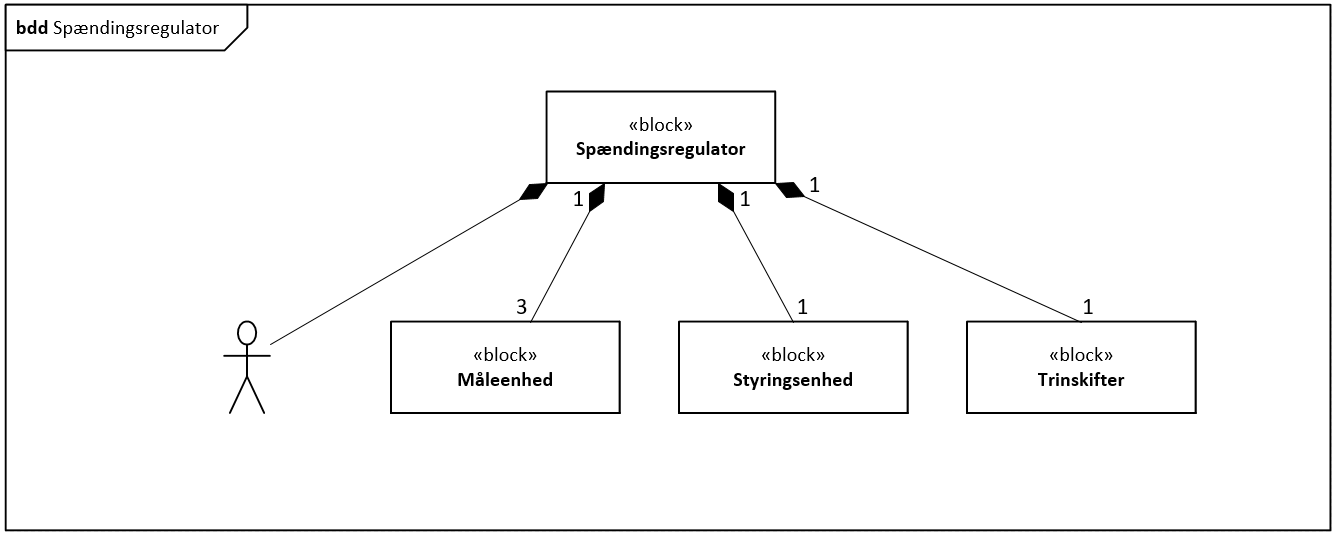
\includegraphics[width=0.9\textwidth]{Figure/BDDSpaendingsregulator}
	\caption{BDD Spændingsregulator}
	\label{fig:BDDSpaendingsregulator}
\end{figure}

\textbf{Måleenhed} står for at måle spænding, strøm og faseforskydningen herimellem. Ligeledes skal denne kunne måle indeholdet af harmoniske frekvenser. Den består af hardware til måling af de nævnte parametre og en PSoC 5. På enheden ligger også en del af behandlingen af rådataet, så dette kan formidles til styringsenheden.

\textbf{Styringsenhed} har til opgave at styre trinskifteren ud fra de data den får fra målenehderne. Den består af en PLC, tl styringen og et HMI, der skal give en bruger overblik over status for distributionslinjen.

\textbf{Trinskifter} er en enhed der kan skifte trin på transformeren ud fra et signal fra styringsenheden. Den består altå af en kontakt for hvert trin, der kan kontrolleres af styringsenheden.
% !TEX root = ../../prj4projektdokumentation.tex
% SKAL STÅ I TOPPEN AF ALLE FILER FOR AT MASTER-filen KOMPILERES 

\section{Intern blok diagram}
På figur \ref{fig:IBDSp} og figur \ref{fig:IBDSt} ses IBD for henholdsvis Spændingsregulator og Styringsenhed. På diagrammerne ses de interne forbindelser i systemet. Under figurne er tilhørende signalbeskrivelser, se tabel \ref{tab:SignalbeskrivelseSp} og tabel \ref{tab:SignalbeskrivelseSt}, der uddyber diagrammerne nærmere.

\begin{figure}[htbp] % (alternativt [H])
	\centering
	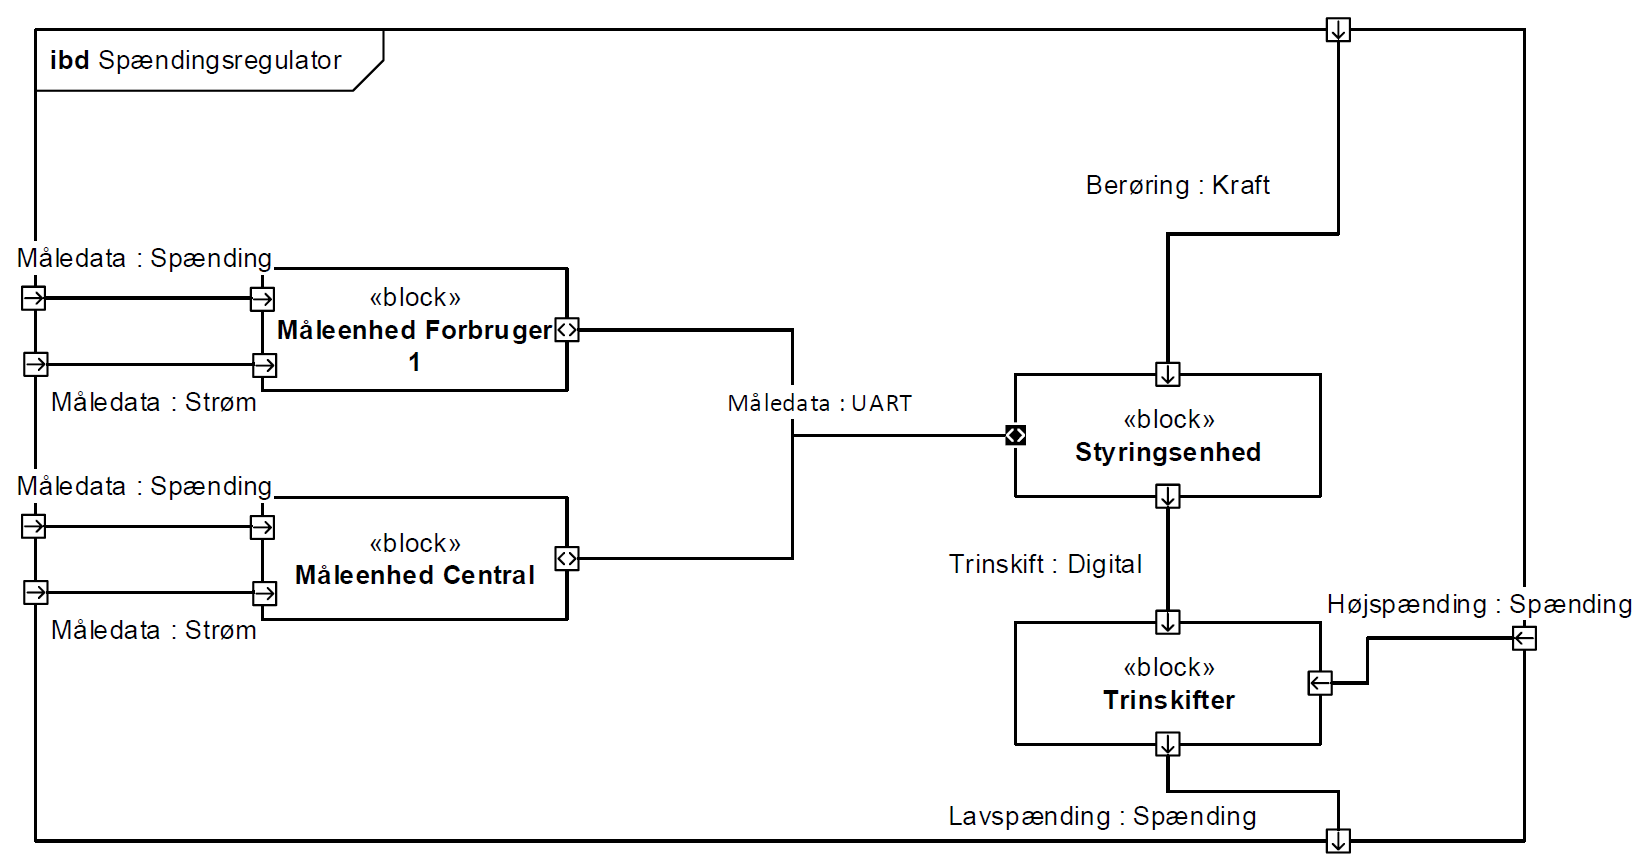
\includegraphics[width=0.8\textwidth]{Figure/IBDSpaendingsregulator1}
	\caption{IBD for Spændingsregulator}
	\label{fig:IBDSp}
\end{figure}

\begin{table}[H]
	\centering
	\begin{tabular}{|l|l|l|l|p{4cm}|}
		\hline
		\textbf{Blok} & \textbf{Navn} & \textbf{Type} & \textbf{Signal} & 
		\textbf{Beskrivelse} \\\hline
		
		\multirow{3}{*}{Måleenhed} 
		& Måledata & Spænding & In & Måledata er spændingsniveauet på distributionslinjen. \\\hhline{~----} 
		& Måledata & Strøm & In & Måledata er strømniveauet på distributionslinjen. \\\hhline{~----} 
		& Måledata & UART & InOut & UART forbindelse til Styringsenhed \\\hline
		
		\multirow{3}{*}{Styringsenhed} 
		& Måledata & UART & Inout & UART forbindelse til Måleenhed \\\hhline{~----} 
		& Berøring & Kraft & In & Tryk på Brugergrænseflade \\\hhline{~----} 
		& Trinskift & Digital & Out & Trinskift er en digital kommando til Trinskifter \\\hline
		
		\multirow{3}{*}{Trinskifter} 
		& Trinskift & Digital & In & Trinskift er en digital kommando fra Styringsenhed. \\\hhline{~----} 
		& Højspænding & Spænding & In & Er spændingen på højspændingssiden af tranformeren. \\\hhline{~----} 
		& Lavspænding & Spænding & Out & Er spændingen på lavspændingssiden af transformeren. \\\hline
	\end{tabular}
	\caption{Signalbeskrivelse for Spændingsregulator}
	\label{tab:SignalbeskrivelseSp}
	
\end{table}


\begin{figure}[htbp] % (alternativt [H])
	\centering
	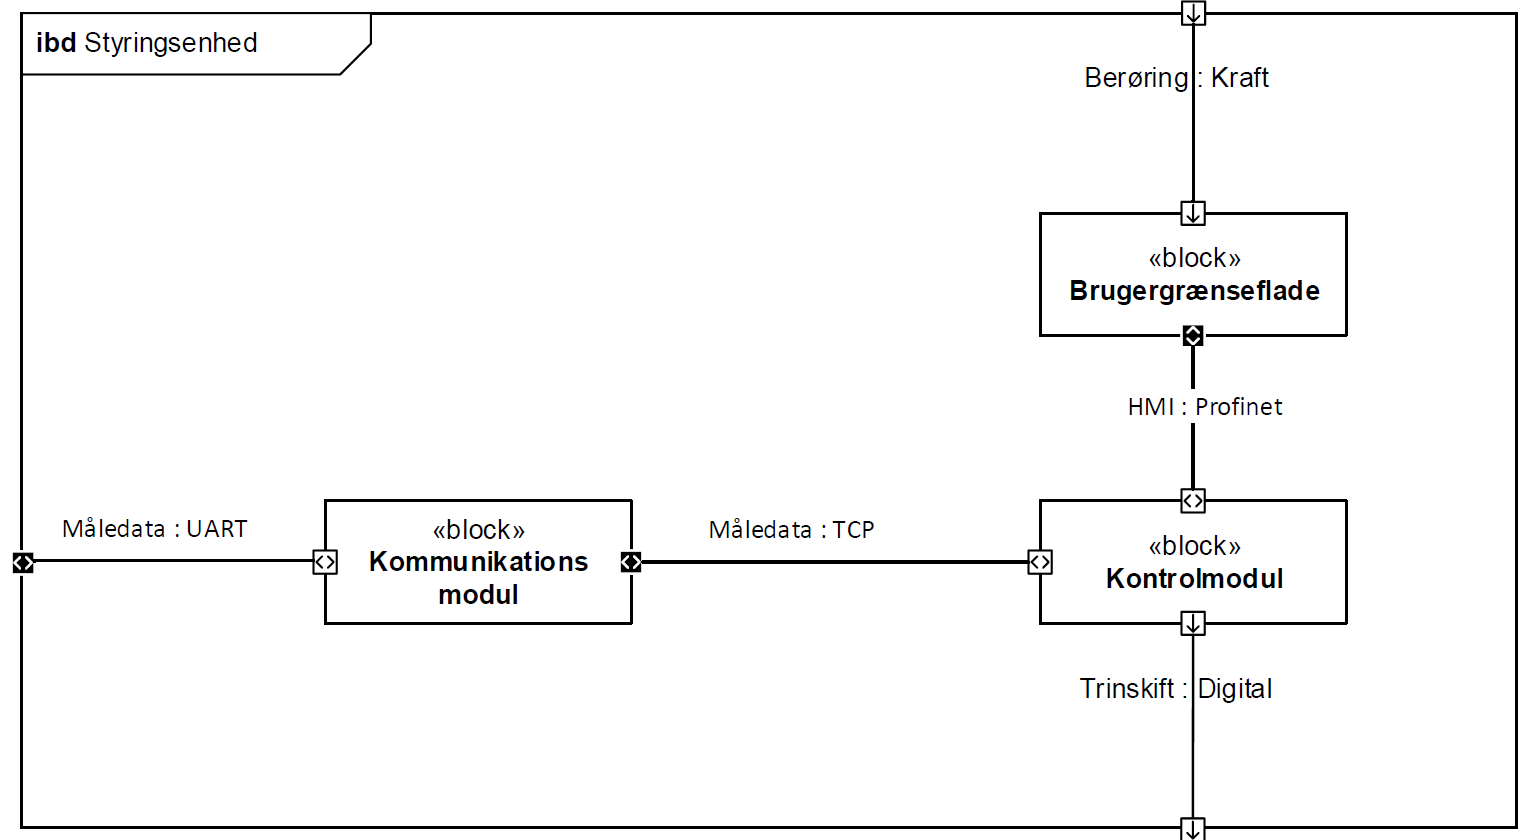
\includegraphics[width=0.8\textwidth]{Figure/IBDStyringsenhed1}
	\caption{IBD for Styringsenhed}
	\label{fig:IBDSt}
\end{figure}

\begin{table}[H]
	\centering
	\begin{tabular}{|l|l|l|l|p{4cm}|}
		\hline
		\textbf{Blok} & \textbf{Navn} & \textbf{Type} & \textbf{Signal} & 
		\textbf{Beskrivelse} \\\hline
		
		\multirow{2}{*}{Brugergrænseflade} 
		& Berøring & Kraft & In & Tryk på Brugergrænseflade \\\hhline{~----} 
		& HMI & Profinet & InOut & Forbindelse til Kontrolmodul \\\hline
		
		\multirow{3}{*}{Kontrolmodul} 
		& HMI & Profinet & InOut & Forbindelse til Brugergrænseflade \\\hhline{~----} 
		& Trinskift & Digital & Out & Trinskift er en digital kommando til Trinskifter \\\hhline{~----} 
		& Måledata & TCP & InOut & TCP forbindelse til Kommunikationsmodul \\\hline
		
		\multirow{2}{*}{Kommunikationsmodul} 
		& Måledata & TCP & InOut & TCP forbindelse til Kontrolmodul \\\hhline{~----} 
		& Måledata & UART & InOut & UART forbindelse til Måleenhed \\\hline
	\end{tabular}
	\caption{Signalbeskrivelse for Styringsenhed}
	\label{tab:SignalbeskrivelseSt}
	
\end{table}


\newpage
% !TEX root = ../../prj4projektrapport.tex
% SKAL STÅ I TOPPEN AF ALLE FILER FOR AT MASTER-filen KOMPILERES 


\section{Allokeringsdiagram}

Herunder ses allokeringsdiagrammet udviklet for systemet. Diagrammet er udviklet for at give et overblik over udviklingen af software og kommunikation i projektet. Et allokeringsdiagram giver et indblik i hvor forskellige dele af projektets funktionalitet skal programmeres, samt hvordan de enkelte enheder kommunikerer sammen. For yderlig beskrivelse af diagrammet se dokumentation\footnote{Projektdokumentation, 5.3, Allokeringsdiagram}.


\begin{figure}[htbp] % (alternativt [H])
	\centering
	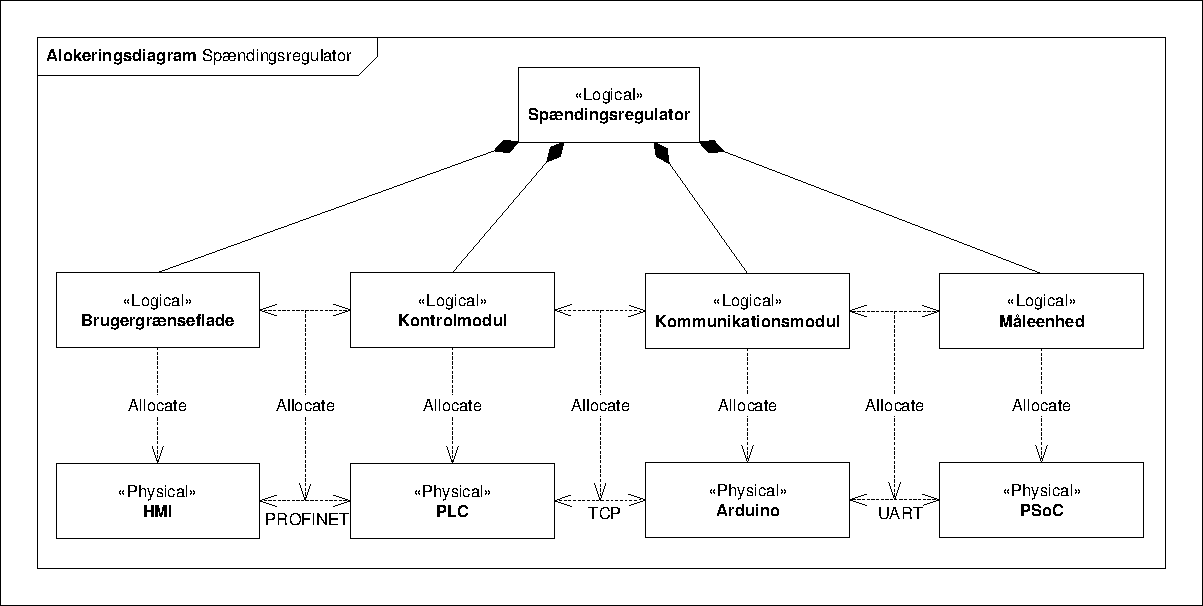
\includegraphics[width=0.8\textwidth]{figure/Allokering.pdf}
	\caption{Allokeringsdiagram for Spændingsregulator}
	\label{fig:Allokering}
\end{figure}
\chapter{Distributionslinje, belastning og trinskifter}
% !TEX root = ../../prj4projektdokumentation.tex

\chapter{Design}

\section{Distributionslinje}
På baggrund af foranalysen er længden af distributionslinjen, der ønskes simuleret, valgt til 60 km. Ud fra datablade for den valgte kabeltype ses at der er vil være 0,1 $\omega$ /km og 0,219 mH/km. For at kunne simulere disse værdier er opbygget et kredsløb med 6,2 $\omega$ modstand i serie med en 13,6 mH spole. 




% !TEX root = ../../prj4projektdokumentation.tex

\section{Belastning}

Med denne distributionslinje og med trinskifteren, der står på 4V trinnet, kan det beregnes hvilken belastning, der vil medføre, at spændingen hos forbrugeren falder til under 10 \% \\ af 4V. Kredsløbet og beregningen ses nedenfor.

\begin{figure}[htbp] % (alternativt [H])
	\centering
	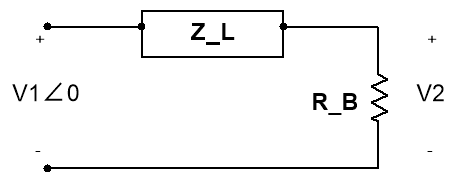
\includegraphics[width=0.4\textwidth]{Figure/Belastningberegning}
	\caption{Kredsløb til beregning af belastning}
	\label{fig:Belastningberegning}
\end{figure}

Først bruges spændingsdelerformlen

\begin{align}
	V2=V1\cdot\frac{R_B}{Z_L+R_B}
\end{align}

\begin{align}
	0,9\cdot\vert V1 \vert = \vert V1\cdot\frac{R_B}{Z_L+R_B} \vert = V1\cdot\frac{R_B}{R_L+jX_L+R_B}
\end{align}

\begin{align}
0,9= \vert \frac{R_B}{R_L+jX_L+R_B} \vert
\end{align}

\begin{align}
	0,9\cdot\vert R_L+jX_L+R_B \vert = \vert R_B \vert
\end{align}

\begin{align}
0,9\cdot\sqrt{(R_L+R_B)^2+X_L^2}=R_B
\end{align}

\begin{align}
(R_L+R_B)^2+X_L^2=\frac{R_B^2}{0,81}
\end{align}

\begin{align}
R_L^2+R_B^2+2\cdot R_L\cdot R_B+X_L^2=\frac{R_B^2}{0,81}
\end{align}

\begin{align}
R_B^2\cdot (1-\frac{1}{0,81})+2\cdot R_L\cdot R_B+X_L^2=0
\end{align}

Værdier indsættes og herved fås:

\begin{align}
R_B^2\cdot (-0,24) +12,4\cdot R_B+18,23=0
\end{align}

Andengrads ligning løses og derved findes den modstandsværdi, der vil give et spændingsfald på 10\%.

\begin{align}
R_B=\frac{-12,4\pm\sqrt{153,76-4\cdot(-0,24)\cdot18,23}}{-0,24\cdot 2}=\frac{-12,4\pm 13,1}{-0,47}=54,3 \Omega
\end{align}

Denne modstandsværdi i det viste kredsløb og med den valgte distributionslinje vil resultere i at spændingen falder under det ønskede niveau som er 4V. Der tages derfor udgangspunkt i denne værdi, men efterfølgende vil belastninger bestemmes ud fra simuleringer i værktøjet Multisim. 

Til implementering af belastninger/forbrugere er på baggrund af foregående beregninger valgt modstande i intervallet 16 $\Omega$ til 100 $\Omega$. Belastninger er placeret i parallel og til hver belastning hører en kontakt, således der let kan skiftes mellem forskellige værdier. Der er desuden monteret pin til forbindelse til distributionslinje og bananstik til forbindelse til 0V på transformeren. Yderligere er der for hver belastning monteret en 1 $\Omega$ modstand således Måleenheden kan overvåge tilstanden hos hver forbruger. Det færdige print med belastninger ses på figur \ref{fig:Belastning1}

\begin{figure}[H] 
	\centering
	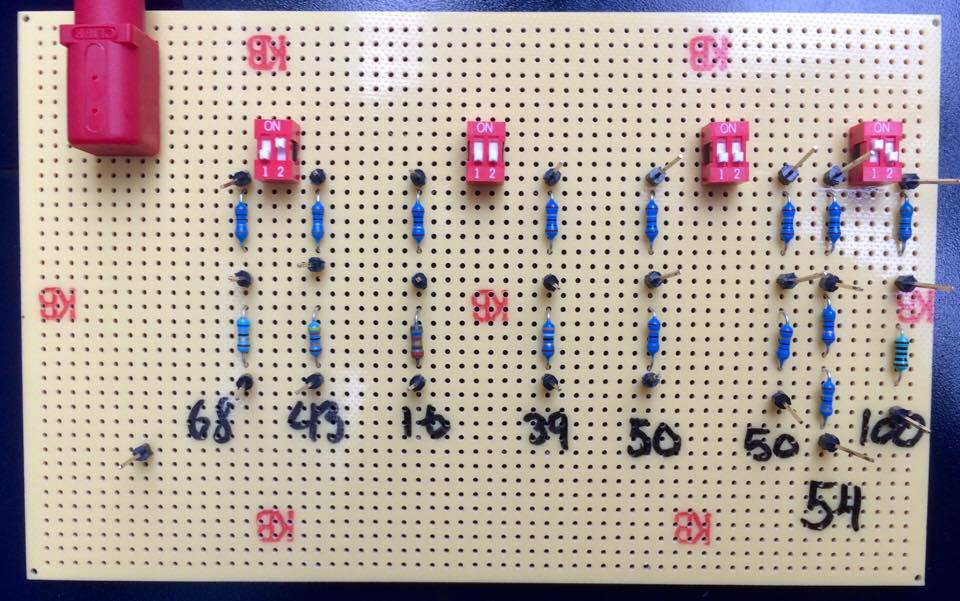
\includegraphics[width=0.7\textwidth]{Figure/Belastningskreds}
	\caption{Færdigt print med belastninger/forbrugere}
	\label{fig:Belastning1}
\end{figure}




% !TEX root =../prj4projektrapport.tex

\section{Trinskifter}

Ved projektets start fik gruppen udleveret en trintransformer\footnote{Projektdokumentation, 6.1, Valg af transformer}. Denne transformer har på primærside 24V og trin af 1V fra 0-8V på sekundærside. Disse forhold afgjorde skaleringen af systemet, se bilag C3 og C4 for billeder af transformer og tilhørende mærkeplade. 

De forskellige trin og dermed spændingsniveauer på sekundærside af transformeren er bestemt af antallet af tilkoblede viklinger. Det ønskede spændingsniveau hos forbrugeren er valgt til 4V, og det er i systemet muligt at skifte mellem trin 4V,5V og 6V på trintransformeren. Disse tre trin gør at muligt at holde spændingen hos forbrugeren på $\pm$10$\%$ af 4V, når belastningen varierer.

\subsection{Design og implementering af relækredsløb}
Til at styre tilkoblingen af trin på transformeren er der designet et relækredsløb. Relæerne er sat til Normally Open og virker som kontakter, der slutter, når relæet trækker. Relæerne skal styres af en PLC, og skal derfor kunne holde til et 24VDC styresignal \footnote{Projektdokumentation, 8.4, Trinskifter}. Det færdige print med relæer ses på figur \ref{fig:Relae}. De sorte banastik kobles til henholdsvis trin 4V,5V og 6V på transformeren. Øverst til ses pin, der kobles til Distributionslinjen. De tre pins nederst til venstre er til styresignal fra PLC og den fjerde er stelforbindelse for PLC. 

\begin{figure}[H]
	\centering
	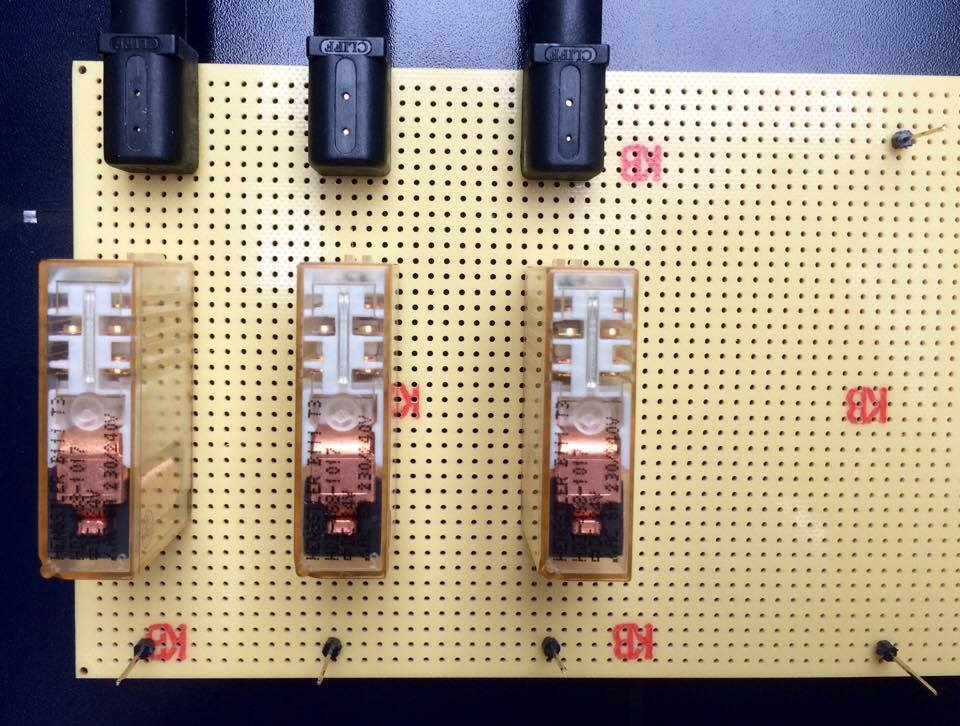
\includegraphics[width=0.6\textwidth]{figure/Relaekredsl}
	\caption{Færdigt print med relæer}
	\label{fig:Relae}
\end{figure}

\subsection{Implementering af Trinsskifter}

Trinskifter består af trintransformer og relækredsløb. På figur \ref{fig:Trinskift} ses implementeringen af denne samt kobling til PLC, Distributionslinje og belastninger.

\begin{figure}[H]
	\centering
	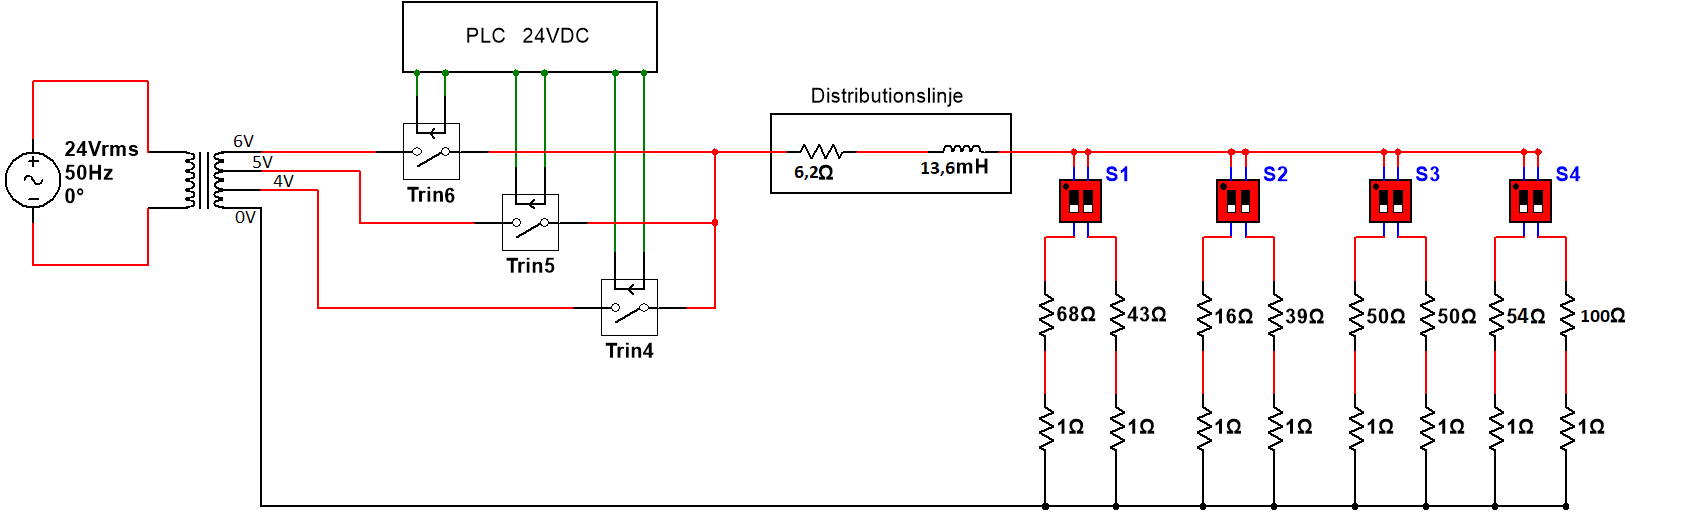
\includegraphics[width=0.8\textwidth]{figure/Trinskiftertegning2}
	\caption{Kredsløbstegning af Distributionslinje, belastninger og Trinskifter}
	\label{fig:Trinskift}
\end{figure}


% !TEX root =../prj4projektrapport.tex

\section{Modultest}


% !TEX root =../prj4projektrapport.tex


\section{Delkonklusion}

I kapitel 5 er overvejelser omkring udvikling, design og implementering af Distributionslinje, Belastning og Trinskifter blevet beskrevet. Der er implementeret en simulering af en 60 km lang distributionslinje med modstand- og spolevirkning, der påvirker spændingsfald og power factor i systemet. Ligeledes er der implementeret belastninger, der kan til- og frakobles for at variere spændingsfaldet over disse. Endeligt er der implementeret en trinskifter i form af en trintransformer og et relækredsløb til skift af trin. På baggrund af modultest kan det konkluderes, at disse enheder giver mulighed for at lave det ønskede proof of concept.


\chapter{Måleenhed}
% !TEX root = ../../prj4projektrapport.tex
% SKAL STÅ I TOPPEN AF ALLE FILER FOR AT MASTER-filen KOMPILERES 

\section{Foranalyse for Styringsenhed}

\subsection{Kontrolmodul og Brugergrænseflade}
Det er en oplagt mulighed at anvende en PLC og et HMI, som Kontrolmodul og Brugergrænseflade i projektet. Dette skyldes at der, som krav til projektet skulle anvendes relevante faglige elementer fra semestrets kurser. Faget Instrumentering og Automatisering(IOA) omhandler netop brugen af PLC og HMI i industrien. Hermed kommer to gode argumenter for PLC og HMI; relevant faglige viden anvendes og i den virkelige verden ville det være oplagt at bruge lignende enheder til et projekt som dette.


PLC'en kan programmeres i flere forskellig sprog. Ladder er dog blevet valgt, fordi det er det mest anvendte i IOA. Desuden er det et krav til projektet at en bruger skal kunne interagere med systemet, hvilket opnåes gennem HMI'et.


Kravet om pålidelig transmission af data mellem udvalgte enheder understøtter også valget af en PLC, da denne indeholder mulighed for LAN kommunikation gennem en RJ-45 port.

\subsection{Kommunikationsmodul}
Det blev hurtigt i projektfasen valgt at der skulle udvikles kommunikation over en LAN forbindelse, da det i projektet var et krav at der skal være pålidelig transmission af data mellem udvalgte enheder. Der blev undersøgt hvilke muligheder der var for at gøre kommunikation over en LAN forbindelse med en microcontroller muligt, da vi allerede havde haft PSoC og Arduino programmering blev der i Embedded Stock bestilt et ethernet shield til hver af disse. Men da Måleenheden bliver implementeret på en PSoC blev det besluttet at prøve at implementere LAN kommunikationen på samme PSoC, som en af Måleenhederne. 


Arduinoen blev holdt som en back-up mulighed, da det er et lettere udviklingsmiljø og samtidig mere populært end PSoC-miljøet, hvorfor der også er mere hjælp at finde om Arduinoen på nettet. Det ville dog være nødvendigt at anvende en anden form for kommunikation mellem Måleenhederne og Arduinoen. 





%Krav: Systemet skal omfatte pålidelig transmission af data mellem udvalgte enheder.
%Komunikationsmodul + shields
%Kommunikationsformer
%Arduino udviklingsmiljø


% !TEX root = ../../prj4projektdokumentation.tex
% !TEX root = ../../prj4projektdokumentation.tex

\section{Indledning}
I dette afsnit beskrives, hvordan Måleenheden er opbygget. Måleenheden er designet til at kunne måle centralt og decentralt, på projektets simulering af transmissionslinje og forbrugere. Der er på netværket forberedt til at der kan tilsluttes måleenheder på forbrugerne. Spændingen kan måles direkte over forbrugeren. På hver forbruger er der tilsluttet 1 1$\Omega$ modstand i serie. På denne modstand måles spændingen, som vil være proportional med strømmen i systemet. Måleenheden er hovedsageligt software, der sampler og udregninger rms, power factor og THD. Der er dog også lavet hardware til at bearbejde signalerne inden PSOC'en.


\section{Hardware}
\subsection{Indledning}
Måleenhedens hardware skal kunne dæmpe spændingen og forstærke strømmen så det ligger inden for PSOC'ens ADC spændingsområde. ADC kan sample signaler mellem 0 og 5Vpp, Det betyder at signalernes offset skal ændres til 2,5V.

\subsection{Diagram}
På figur \ref{fig:MaalDiagram} ses diagrammet for det hardware der bruges til at dæmpe spændingen, forstærke strømmen og hæve offsettet.

\begin{figure}[H] % (alternativt [H])
	\centering
	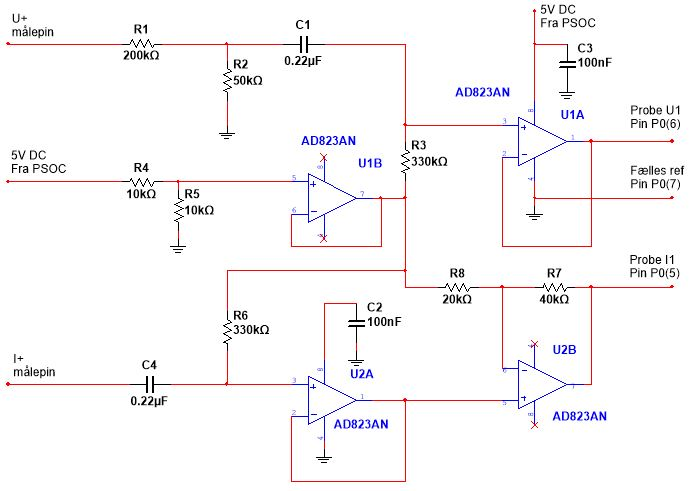
\includegraphics[width=\textwidth]{Figure/MaalHardware}
	\caption{Hardware diagram}
	\label{fig:MaalDiagram}
\end{figure}


\subsubsection{Spændingsmåler}
For at kunne måle den maksimale spænding på 8V rms, dvs.

\begin{align}
Vpp = 8V*\sqrt{2} = 11,3Vpp
\end{align}

Den mindste dæmpning skal derfor være:

\begin{align}
min\_daemp = \dfrac{11.3}{5} = 2,26 gange
\end{align}

Dette er valgt realiseret med en spændingsdeler ved R1 og R2. De dæmper med 3 gange og niveauet kommer derfor indenfor marginen.
Derefter bliver offsettet hævet ved hjælp af signalet fra U1B. Til sidst føres signalet gennem spændingsfølgeren U1A for at sikre spændingen.

\subsubsection{Strømmåling}
Strømmålingen laves ved at måle spændingen over en 1$\Omega$ modstand. Modstanden sidder placeret ved belastningen. Iht. ohmslov vil det give strømmen i systemet
.
\begin{align}
	I = \dfrac{U}{1\Omega} = U
\end{align}

Første Opamp U2A ved strømmålingen bruges til at hæve DC offset til 2,5V. Opamp U2B bruges til at forstærke strømmen så der kommer bedre præcision på målingen. Den maskimale forstærkning, for at den passe indenfor PSOC'ens ADC sample område bliver derfor:

Den maksimale Ipp der vil kunne måles:
\begin{align}
Ipp = 0,5*\sqrt{2} = 0,71A
\end{align}

Maksimale forstærkning:
\begin{align}
maks\_forstaerkning = \dfrac{5}{0,71} = 7
\end{align}
Denne forstærkning ses realiseret vha. modstand R7 og R8.  

\subsubsection{PSOC tilslutning}
Spændingen og strømmen bliver målt til den fælles nul i systemet, der bliver koblet på hardwarens stel forbindelse. Spænding, strøm og stel forbindelsen tilsluttes PSOC'en, som vist på figur \ref{fig:MaalDiagram}.





% !TEX root = ../../prj4projektrapport.tex
% SKAL STÅ I TOPPEN AF ALLE FILER FOR AT MASTER-filen KOMPILERES 

\subsection{Software}
I dette afsnit vil design og implementering af softwaren på PSOC blive beskrevet. Herunder ADC konvertering, Fourier beregninger og  UART kommunikation. For detaljeret beskrivelse af softwaren henvises til dokumentationen\footnote{Projektdokumentation, 9.2, Software}

\subsubsection{Overordnet beskrivelse}
Det overordnede flow i koden er vist i Figur \ref{fig:MEflowchart}, og vil blive beskrevet i den følgende tekst.  

Ved start af Måleenheden sker der en række initieringer af interrupts og blokkald. Herefter ender koden i en uendelig loop, uden aktivitet. Ved modtagelse af data over UART forbindelsen aktiveres en interruptrutine, hvor hovedparten af kodens funktionalitet er allokeret. 
Afhængigt af hvilken karakter der er modtaget på UART forbindelsen udførers forskellige instruktioner. I følge protokollen for UART-forbindelsen modtages karakterene A-B-C-D, i rækkefølge, se dokumentationen\footnote{Projektdokumentation, 7.2, UART protokol}
Når den første karakter A er modtaget påbegynder måleneheden sampling af signalerne, hvorefter værdien for strøm sendes tilbage over UART forbindelsen. Herefter afventes de resterende modtage interrupt, som giver anledning til at spænding, THD, og power faktor sendes til Styringsenheden. 
\begin{figure}[h] % (alternativt [H])
	\centering
	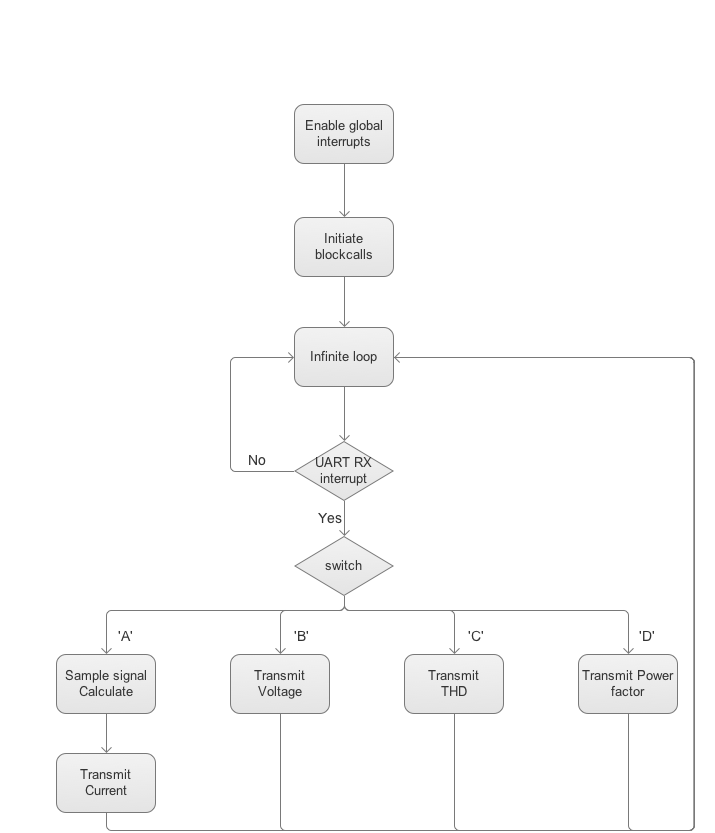
\includegraphics[width=0.7\textwidth]{Figure/MEflowchart.png}
	\caption{Overordnet flowchart for software på Måleenhed}
	\label{fig:MEflowchart}
\end{figure}





% !TEX root = ../../prj4projektrapport.tex
% SKAL STÅ I TOPPEN AF ALLE FILER FOR AT MASTER-filen KOMPILERES 

\subsubsection{Analog til digital konvertering}
Måleenheden omsætter to analoge spændingssignaler til digitale værdier, som kan behandles af softwaren på PSOC. Denne konvertering foretages af en Delta Sigma Analog to Digital Converter (ADC), som er indstillet med en opløsning på 16bit og en samplefrekvens på 41,67kHz. Denne samplefrekvens er meget højere end minimumskravet på 500Hz jf. Shannons samplingssætning. Med den samplefrekvens vil datamængden, der skal behandles i Fourier transformation blive alt for stor. Derfor er samplefrekvensen nedsat ved at indsætte et delay i koden efter hvert andet sample. Se dokumentationen\footnote{Projektdokumentation, 9.2.2, Analog til digital konvertering} for udregning af delayets størrelse. Med delayet er samplefrekvensen nedsat til 3,2kHz for hvert signal, hvilket svarer til 64 samples pr. periode af 50Hz signalet. Da der samples to signaler skiftevis vil ADC'ens reelle samplefrekvens være 6,4kHz, og der vil være en forsinkelse mellem samplingen af de to signaler. Ved beregning af power factor er der set bort fra denne forsinkelse, da den ikke har afgørende betydning for resultatet.  

% !TEX root = ../../prj4projektdokumentation.tex

\section{Software}


% !TEX root = ../../prj4projektrapport.tex
% SKAL STÅ I TOPPEN AF ALLE FILER FOR AT MASTER-filen KOMPILERES 

\subsubsection{Beregningsfunktioner}
For at beregne de ønskede værdier er der lavet en række funktioner der kan beregne disse. Disse funktioner er kort beskrevet herunder. Yderlig information findes i dokumentation\footnote{Projektdokumentation, 9.2.4, Beregning af rms og power faktor}

\textbf{Rms:}
Funktionen modtager et array af absolutte værdier for et signal og beregner rms værdien, ved den frekvensbin der passer til 50Hz.

\textbf{Power faktor:}
Funktionen beregner vinklen for strøm og spænding for derefter at beregne power factor ved at tage cosinus til vinkel differencen. Funktionen tager ikke højde for om strømmen er leading eller lagging.

\textbf{THD:}
Beregningen af, og baggrunden for THD, er beskrevet i Afsnit \ref{sec:THD}. Den beregning der laves i PSoC, medregner kun indholdet af de fire første harmoniske i signalet. Formlen der anvendes i softwaren er givet i Ligning \ref{eq:THDsoft}.
\begin{align}
\label{eq:THDsoft}
THD = \dfrac{\sqrt{V_2^{2}+V_3^{2}+V_4^{2}+V_5^{2}}}{V_{1}}
\end{align}
 

\subsubsection{UART kommunikation}
Kommunikationen mellem Måleenheden og Styringsenheden er allokeret på en UART forbindelse, se Figur \ref{fig:Allokering} for overordnet allokeringsdiagram. UART forbindelsen transmitterer 16bit værdier for strøm, spænding, THD og power factor. Værdierne deles inden transmissionen op i to pakker af 8bit, og samles igen i Styringsenheden. Protokol og indstilling af UART forbindelsen er beskrevet i dokumentationen\footnote{Projektdokumentation, 7.2, UART protokol}.





% !TEX root = ../../prj4projektdokumentation.tex

\subsection{Kalibrering af måleenhed.}

Efter test af funktionaliteten af Måleenheden laves en kalibrering, for at fjerne det offset, som er opstået i forbindelse med forstærkning/dæmpning af signal i hardwaren. 

\subsubsection{Måleopstilling}

Til kalibrering af måleenheden er anvendes en funktionsgenerator, til at lave sinussignalet, som forbindes direkte til måleenheden. Til korrekt måling af spændingsværdier anvendes oscilloskop, som her antages for værende ideel. Måleenheden er tilsluttet en PC og kører i debug-mode, så værdierne for strøm og spænding kan aflæses. 
\begin{figure}[H]
	\centering
	\begin{minipage}[b]{0.48\textwidth}
		\centering
		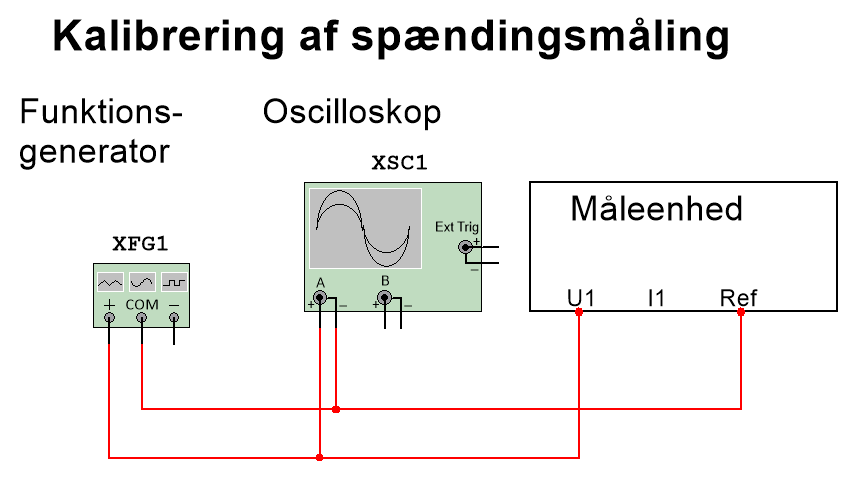
\includegraphics[width=1.00\textwidth]{Figure/MEkalibreringU} % Venstre billede
	\end{minipage}
	\hfill
	\begin{minipage}[b]{0.48\textwidth}
		\centering
		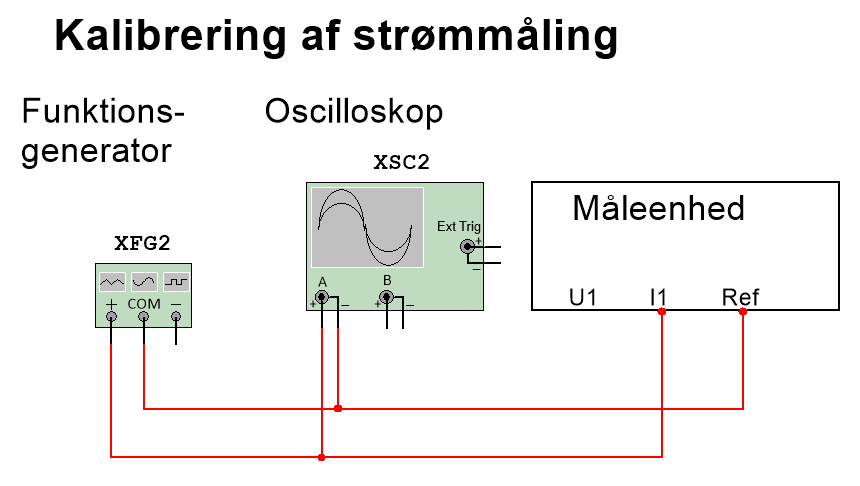
\includegraphics[width=1.00\textwidth]{Figure/MEkalibreringI} % Højre billede
	\end{minipage}
	\\ % Figurtekster og labels
	\begin{minipage}[t]{0.48\textwidth}
		\caption{Måleopstilling for kalibrering af spændingsmåling} % Venstre figurtekst og label
		\label{fig:MEkalibreringU}
	\end{minipage}
	\hfill
	\begin{minipage}[t]{0.48\textwidth}
		\caption{Måleopstilling for kalibrering af strømmåling} % Højre figurtekst og label
		\label{fig:MEkalibreringI}
	\end{minipage}
\end{figure}

\subsubsection{Fremgangsmåde}

Der laves to måleserier, for henholdsvis spænding- og strømmåling. Strømmålingen er baseret på en spændingsmåling over en $1\Omega$ modstand, hvilket betyder at spændingsfaldet over modstanden lig med strømmen. Derfor kalibreres strømmålingen med et spændingssignal, på samme måde som spændingsmålingen. Måleenheden er lavet til at måle en spænding mellem 0-8Vrms og en strøm mellem $\SI{500}{\milli\ampere}$, så der laves målinger i dette område med intervaller på $\SI{500}{\milli\volt}$ og $\SI{50}{\milli\volt}$.

Der forventes at se en lineær sammenhæng mellem faktiske spændinger og værdierne fra debuggeren på Måleenheden. Ved at finde hældningen på denne sammenhæng findes den konstant, som skal ganges på resultatet i måleenheden, for værdierne passer med den faktiske spænding. 

\subsubsection{Resultater}
Måleresultaterne fra kalibreringen findes i Tabel \ref{tab:MEkalibrering}. Sammenhængen mellem faktiske spændinger og værdierne i Måleenheden er vist i Figur \ref{fig:MEgraf}.

% Table generated by Excel2LaTeX from sheet 'Ark1'
\begin{table}[htbp]
	\centering
	\caption{Måleresultater for kalibrering af Måleenhed.}
	\begin{tabular}{rrrrr}
		\toprule
		& \multicolumn{1}{l}{Faktiske værdier} &       & \multicolumn{1}{l}{Måleenhed} &  \\
		\multicolumn{1}{l}{Måling nr. } & \multicolumn{1}{l}{Spænding} & \multicolumn{1}{l}{Strøm} & \multicolumn{1}{l}{Spænding } & \multicolumn{1}{l}{Strøm} \\
		\midrule
		1     & 0     & 0     & 0     & 0 \\
		2     & 500   & 50    & 93    & 152 \\
		3     & 1000  & 100   & 185   & 308 \\
		4     & 1509  & 150   & 276   & 462 \\
		5     & 2008  & 199   & 368   & 610 \\
		6     & 2503  & 250   & 460   & 764 \\
		7     & 2999  & 299   & 553   & 912 \\
		8     & 3502  & 350   & 645   & 1069 \\
		9     & 3808  & 399   & 699   & 1216 \\
		10    & 4006  & 450   & 736   & 1370 \\
		11    & 4505  & 500   & 828   & 1518 \\
		12    & 5000  &       & 918   &  \\
		13    & 5499  &       & 1009  &  \\
		14    & 6000  &       & 1111  &  \\
		15    & 6505  &       & 1197  &  \\
		16    & 7006  &       & 1284  &  \\
		\bottomrule
	\end{tabular}%
	\label{tab:MEkalibrering}%
\end{table}%

\begin{figure}[H]
	\centering
	\includegraphics[width=0.80\textwidth]{Figure/MEkalibreringgraf}
	\caption{Sammenhæng mellem faktiske spændinger og værdier i Måleenheden.}
	\label{fig:MEgraf}
\end{figure}

Faktoren som skal ganges på resultatet i Måleenheden findes for henholdsvis spænding og strøm, ved hældningen af de to lineære funktioner på Figur \ref{fig:MEgraf}.
\begin{align}
	a_{U} = 5,4391
\end{align}
\begin{align}
a_{I} = 0,3291
\end{align}
% !TEX root =../prj4projektrapport.tex

\section{Modultest}


% !TEX root =../prj4projektrapport.tex


\section{Delkonklusion}

I kapitel 5 er overvejelser omkring udvikling, design og implementering af Distributionslinje, Belastning og Trinskifter blevet beskrevet. Der er implementeret en simulering af en 60 km lang distributionslinje med modstand- og spolevirkning, der påvirker spændingsfald og power factor i systemet. Ligeledes er der implementeret belastninger, der kan til- og frakobles for at variere spændingsfaldet over disse. Endeligt er der implementeret en trinskifter i form af en trintransformer og et relækredsløb til skift af trin. På baggrund af modultest kan det konkluderes, at disse enheder giver mulighed for at lave det ønskede proof of concept.


\chapter{Design af Styringsenhed}
% !TEX root =../prj4projektrapport.tex

Formålet med dette projekt er at løse følgende problemformulering; \textit{Når belastningerne i et distributionssystem ændres, vil spændingsniveauet variere. Det er vigtigt, at spændingsniveauet holdes stabilt. Hvordan sikres dette?}
Udgangspunktet for problemstillingen er det lovmæssige krav, der siger, at spændingsforsyningen hos danske forbrugere altid skal ligge på 230V $\pm$10$\%$ \cite{Sikkerhedsstyrelsen}. Det ønskes at undersøge udfordringerne ved dette samt at komme med et bud på, hvordan denne problemstilling løses bedst muligt, både som elnettet ser ud i dag, men også i fremtiden. 

For at kunne arbejde med problemformuleringen og undersøge dens aktualitet, valgte projektgruppen at tage kontakt til energiselskabet Eniig. Det viste sig, at der på nuværende tidspunkt ikke foretages regulering på lavspændingsnettet, men i stedet på 60/10 kV transformere. Projektgruppen fandt det derfor interessant at undersøge mulighederne for regulering på lavspændingsnettet og eventuelle fordele og fremtidsaspekter ved dette.

I dette projekt vil fokus derfor være på den del af nettet, der går fra distributionstransformer og ud til forbrugere. For at sikre et stabilt spændingsniveau ønskes det at kunne overvåge tilstanden på distributionslinjen, ikke kun ved transformeren, men også ved hver enkelt forbruger. Det samlede system, der fremstilles i projektet betegnes som Spændingsregulator. Med denne ønskes det at lave et proof of concept i forhold til problemformuleringen. På grund af tilgængelighed af komponenter og udstyr vil prototypen for Spændingsregulator blive skaleret ned. 

For at belyse problemstillingen vil der i dette projekt blive lavet en simulering af en distributionslinje samt belastninger, der skal simulere forbrugere på linjen. Projektet vil desuden bestå af en trintransformer, der giver mulighed for at variere spændingsniveauet til linjen og forbrugerne på sekundærsiden af transformeren.

Til justering af spændingsniveauet, er det nødvendigt at kende til de aktuelle værdier for spændingen både centralt ved trintransformeren og decentralt ved forbrugerne. Af denne grund implementeres enheder til måling af spændingen. Det ønskes desuden at kende til systemets power factor, og derfor skal strømmen også måles. Et eventuelt indhold af harmoniske kan føre til unødig belastning og opvarmning af transformere, og det er derfor fornuftigt at kende til indholdet af harmoniske, og denne parameter skal også måles.
For at kunne holde et ønsket spændingsniveau vil der i projektet implementeres en enhed til regulering af trin på transformeren.

\begin{figure}[H]
	\centering
	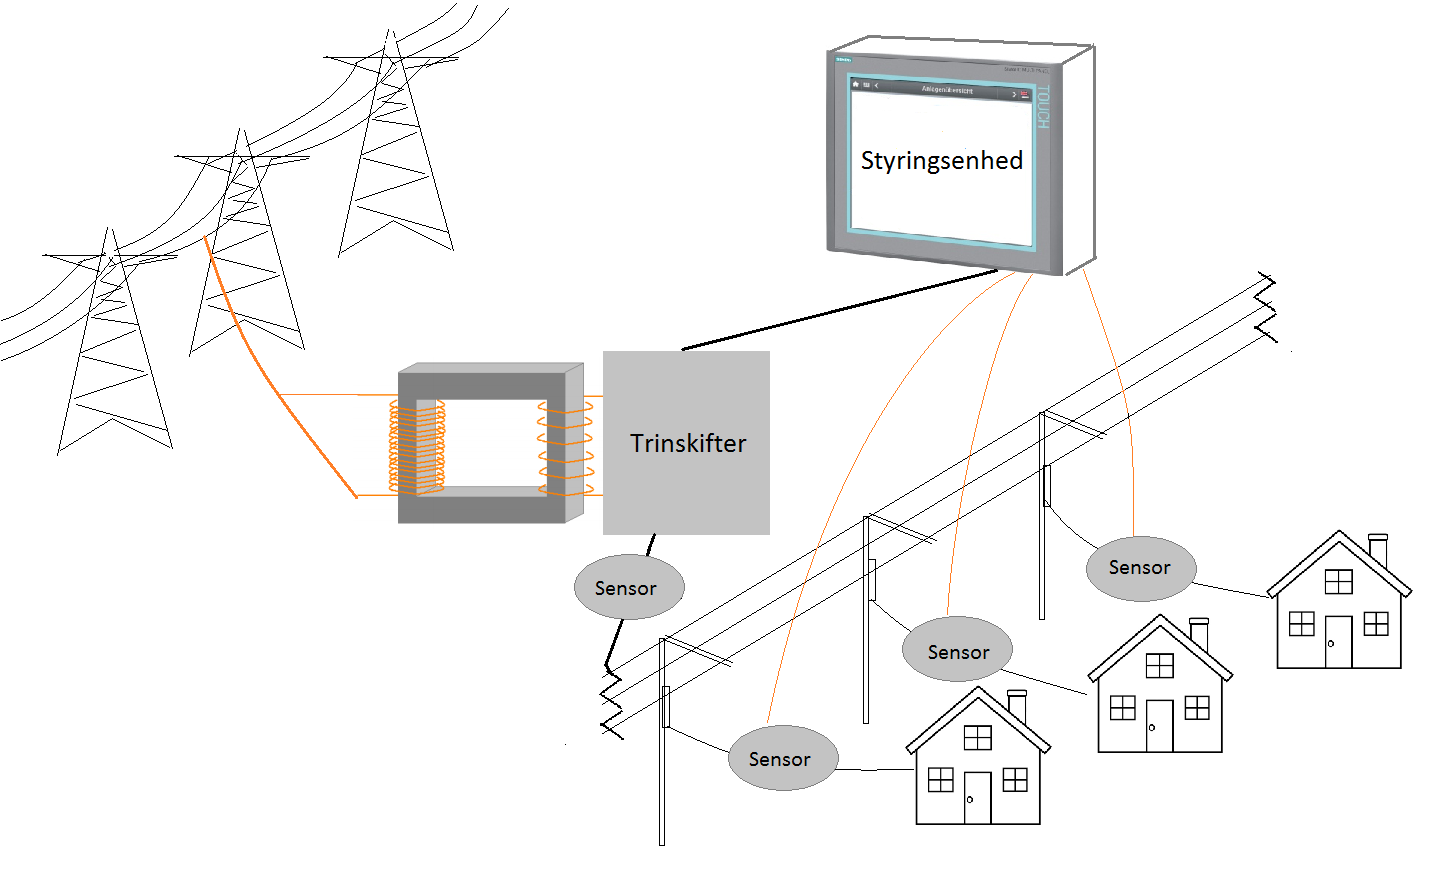
\includegraphics[width=1\textwidth]{figure/RigtBillede}
	\caption{Visuel fremstilling af Spændingsregulator}
	\label{fig:Rigtbillede}
\end{figure}

På figur \ref{fig:Rigtbillede} ses en illustration, der giver oveblik over Spændingsregulatoren. Billedet viser trintransformeren, der forsyner distributionslinjen, sensorer, der måler aktuelle værdier på linjen og en styringsenhed, der regulerer trintransformeren på baggrund af disse værdier. 
% !TEX root = ../../prj4projektrapport.tex
% SKAL STÅ I TOPPEN AF ALLE FILER FOR AT MASTER-filen KOMPILERES 

\section{Foranalyse for Styringsenhed}

\subsection{Kontrolmodul og Brugergrænseflade}
Det er en oplagt mulighed at anvende en PLC og et HMI, som Kontrolmodul og Brugergrænseflade i projektet. Dette skyldes at der, som krav til projektet skulle anvendes relevante faglige elementer fra semestrets kurser. Faget Instrumentering og Automatisering(IOA) omhandler netop brugen af PLC og HMI i industrien. Hermed kommer to gode argumenter for PLC og HMI; relevant faglige viden anvendes og i den virkelige verden ville det være oplagt at bruge lignende enheder til et projekt som dette.


PLC'en kan programmeres i flere forskellig sprog. Ladder er dog blevet valgt, fordi det er det mest anvendte i IOA. Desuden er det et krav til projektet at en bruger skal kunne interagere med systemet, hvilket opnåes gennem HMI'et.


Kravet om pålidelig transmission af data mellem udvalgte enheder understøtter også valget af en PLC, da denne indeholder mulighed for LAN kommunikation gennem en RJ-45 port.

\subsection{Kommunikationsmodul}
Det blev hurtigt i projektfasen valgt at der skulle udvikles kommunikation over en LAN forbindelse, da det i projektet var et krav at der skal være pålidelig transmission af data mellem udvalgte enheder. Der blev undersøgt hvilke muligheder der var for at gøre kommunikation over en LAN forbindelse med en microcontroller muligt, da vi allerede havde haft PSoC og Arduino programmering blev der i Embedded Stock bestilt et ethernet shield til hver af disse. Men da Måleenheden bliver implementeret på en PSoC blev det besluttet at prøve at implementere LAN kommunikationen på samme PSoC, som en af Måleenhederne. 


Arduinoen blev holdt som en back-up mulighed, da det er et lettere udviklingsmiljø og samtidig mere populært end PSoC-miljøet, hvorfor der også er mere hjælp at finde om Arduinoen på nettet. Det ville dog være nødvendigt at anvende en anden form for kommunikation mellem Måleenhederne og Arduinoen. 





%Krav: Systemet skal omfatte pålidelig transmission af data mellem udvalgte enheder.
%Komunikationsmodul + shields
%Kommunikationsformer
%Arduino udviklingsmiljø


% !TEX root = ../../prj4projektrapport.tex
% SKAL STÅ I TOPPEN AF ALLE FILER FOR AT MASTER-filen KOMPILERES 

\section{Kontrolmodul}

Kontrolmodulet består af en Siemens PLC S7-1200 med signalmodulet AQ1x12BIT. Det kan tilgås gennem en switch af typen CSM 1277.
Softwaren består af to dele; en kommunikationsdel med interface til kommunikationsmodulet og en kontroldel med interface til Trinskifter. Den detaljerede gennemgang af softwaren kan findes i dokumentationen.\footnote{Projektdokumentation, 10.1, Kontrolmodul} Her vil i stedet blive lagt fokus på de overvejelser, der har været undervejs i designet af Kontrolmodulet.
Kontrolmodulet er lavet i en OB, der looper. Heri er placeret fire FC'er, der er oprettet i forbindelse med kommunikationen og den FB, der er fremstillet til styring af Trinskifter.

\subsection{Kommunikation}
Datatransmission til Kontrolmodulet er en vigtig del af projektet, da dette forbinder sensorer i form af Måleenhederne med aktuatorer i form af Trinskifter. Derfor er der blevet lagt mange overvejelser i, hvordan kommunikationen skulle etableres.


Først og fremmest skulle flere Måleenheder kunne kommunikere med det samme kontrolmodul, derfor var en switch i overvejelser, grundet der kun er én fri RJ-45 port på PLC'en. Dette var ikke umiddelbart muligt at fremskaffe hos Embedded Stock. For mere om løsningerne på dette, se afsnit \ref{Kommunikationsmodul}.


Næste beslutning gik på valget af protokol til Ethernet kommunikation. TCP var det oplagte valg for at sikre pålidelig kommunikation, selvom UDP også var en kendt protokol fra faget Internet kommunikationsnetværk(IKN).


Udvilingsværktøjet TIA Portal V13 har gode muligheder for at sætte TCP kommunikation op til forskellige ikke Siemens produkter gennem dets open user communication. Først blev blokkene TSEND\_C og TRCV\_C forsøgt anvendt. Disse blokke har dog indbygget funktionalitet i forbindelse med at oprette og nedlægge forbindelsen, hvilket var uhensigtmæssigt, når der skulle være en flydende datastrøm. Det endelige valg blev derfor blokkene TCON, TDISCON, TSEND og TRCV, hvor man som programmør kan styre oprettelse og nedlæggelse af forbindelsen med TCON og TDISCON. På figur \ref{fig:TSEND} ses blokken TSEND som et eksempel på open user communication blokkene.

\begin{figure}[H] % (alternativt [H])
	\centering
	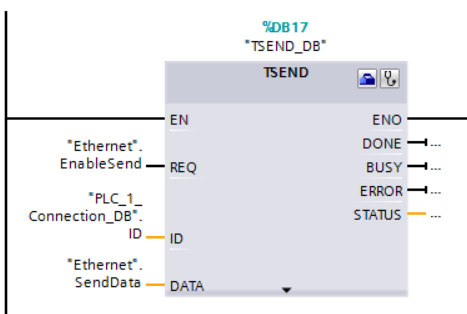
\includegraphics[width=0.5\textwidth]{Figure/TSEND}
	\caption{Blokken TSEND}
	\label{fig:TSEND}
\end{figure}


Med en pålidelig og testet TCP kommunikation var de næste overvejelser angående styringen af disse blokke. Her blev det besluttet, at et client/server forhold ville være bedst. Kontrolmodulet er i den sammenhæng client og skal forespørge data fra serveren, Kommunikationsmodulet.
Da systemet ikke er et beskyttelsessystem, kræver det ikke hurtig reaktion mellem sensor og aktuator. Derfor blev det valgt, at det kun var nødvendigt at opdatere data hvert 2 sekunder. Dette blev realiseret med to separate netværk; et tilknyttet FC'en med TSEND og et tilknyttet FC'en med TRCV. På figur \ref{fig:ValgAfEnhedSend} ses netværket tilknyttet TSEND.

\begin{figure}[H] % (alternativt [H])
	\centering
	\includegraphics[width=1\textwidth]{Figure/valgAfEnhedSend}
	\caption{Netværket der styrer hvilken enhed der forespørges data fra}
	\label{fig:ValgAfEnhedSend}
\end{figure}

FC'er er valgt, da tanken var at hukommelsen skulle ligge andetsteds i koden. Det er dog blevet nødvendigt at oprette en global DB for at kunne styre variable i forbindelse med styring af kommunikationen. For yderlige uddybelse, se dokumentationen\footnote{Projektdokumentation, 10.1.1, TCP kommunikation}.


Det er vigtigt at pointere, at systemet skal være nemt at udvide til at understøtte mange Måleenheder i den virkelige verden. Det vil udvide tiden, det tager at eksekvere programmet, men er nemt, da der ikke skal ændres i selve kommunikationen, men kun i de netværk, der styrer kommunikationen, hvor der her skal tilføjes flere forgreninger.

\subsection{Styring af Trinskifter}

Angående styring af Trinskifteren blev det tidligt besluttet at benytte dens analoge 24VDC udgange på Q0.6, Q0.7 og Q1.0 til styringen af relæerne på Trinskifter. Disse udgange bliver dog styret med et logisk højt (24VDC) eller lavt(0V) signal. Der henvises til Trinskifter for mere om relækredsløbet, se afsnit \ref{sec:relae}.
Samtidig er projektet proof of concept, så det er kun spændingsmålinger fra én forbruger, der vil blive reguleret med hensyn til. Dette simplificerer den FB, der udvikles til denne styring væsentligt, da der kun er et input. På \ref{fig:GraphTrinskifterPLC} ses et diagram over sekvenserne og flowet imellem dem for FB'en Trinskifter.

\begin{figure}[H] % (alternativt [H])
	\centering
	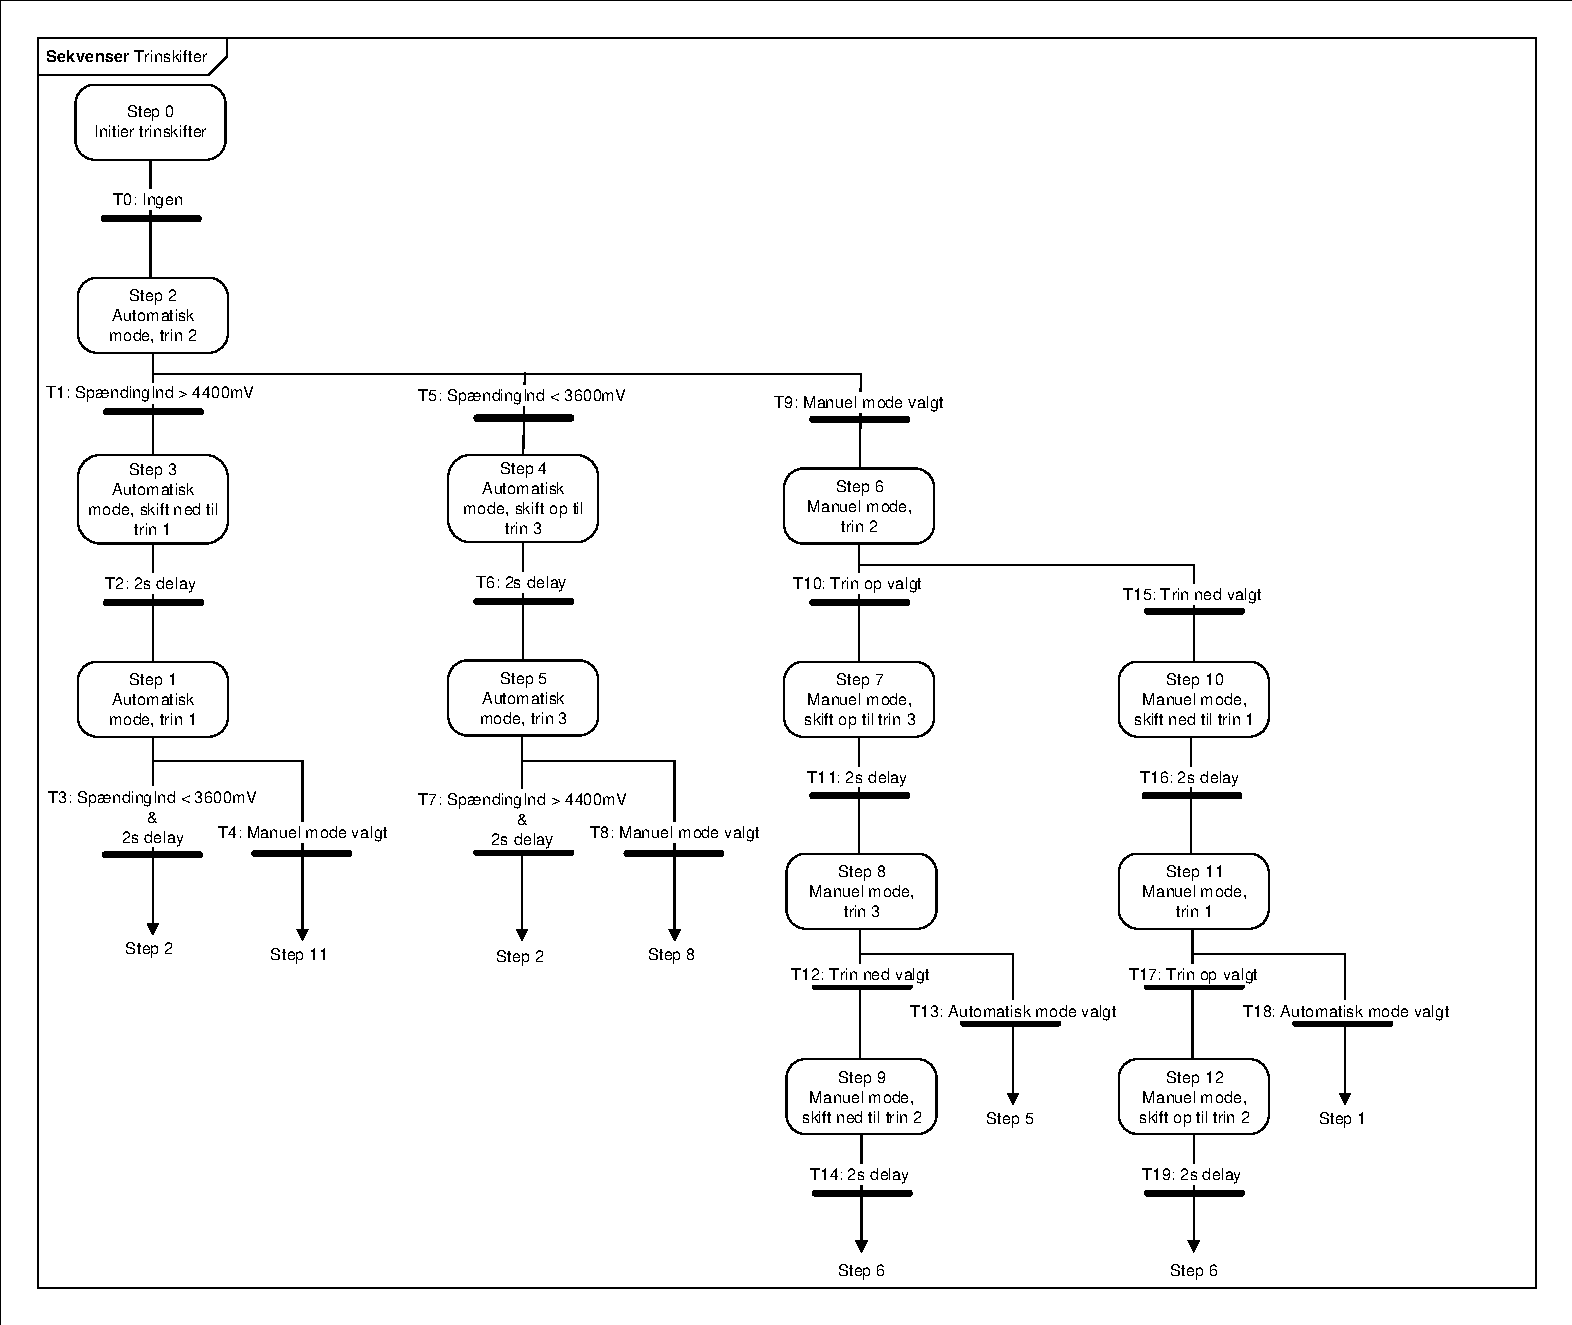
\includegraphics[width=1\textwidth]{Figure/GraphTrinskifterPLC}
	\caption{Diagrammet viser FB'en Trinskifters sekvenser}
	\label{fig:GraphTrinskifterPLC}
\end{figure}

Første tanke i forhold til denne blok var, at den hovedsageligt skulle være automatiseret. Derfor er det besluttet, at koden blev skrevet som sekventiel, hvor en lokal static Step står for at styre, hvilken sekvens der er aktiv. Dette sikrer også imod fejl, da systemet har få muligheder videre fra hvert step. Et sikkert system var også et af de vigtige punkter, hvilket bl.a. er opnået ved at opdele koden i sekvenser af trin og trinskift. Der er 3 trin, som hver især er tilknyttet en af udgangene på PLC'en. For trin 2 er der både mulighed for et trinskift op og ned, mens der for ydertrinene kun kan skiftes ned/op til trin 2. Det er kun, når koden er i et trin, at man kan skifte mellem automatisk og manuel tilstand. I automatisk mode er der dog to undtagelser i trin 1 og trin 3, hvor trinskiftet er lagt sammen med trinet. Disse trinskift burde have været flyttet til deres egen sekvens for at undgå at et trinskift og et tilstandsskift kan forekomme samtidigt.


I første udkast til blokken var der ikke taget højde for at programmet blev eksekveret hurtigere end data blev opdateret, derfor kunne programmet nå at skifte flere trin på den samme måling, hvilket vil skabe et ustabilt system, for når det havde lavet et dobbeltskift, vil det så få en ny måling, der indikerer skift i modsat retning. Denne fejl er fjernet ved at indsætte et delay, når systemet kommer i et nyt trin, da der hentes ny data hvert 2 sekunder, er dette delay sat til 2,5 sekunder.


En vigtig pointe at få med er, at forbrugeren aldrig må miste forsyning. Så et trinskift indebærer et overlap imellem de trin, der skiftes fra og til på 2 sekunder. Herved er der altid forsyning på distributionslinjen. Selve overlappet set fra trintransformeren uddybes i afsnit \ref{sec:ImpTrinskift}.
For mere om styringen af trinskifteren, se dokumentationen.\footnote{Projektdokumentation, 10.1.2, Styring af Trinskifteren.}

% !TEX root = ../../prj4projektrapport.tex
% SKAL STÅ I TOPPEN AF ALLE FILER FOR AT MASTER-filen KOMPILERES 


\section{Brugergrænseflade}

Brugergrænsefladen i dette projekt er designet på en HMI KTP 600. Den kan tilgås gennem en switch af typen CSM 1277. I dette afsnit vil overvejelser omkring HMI'et blive gennemgået, koden og opsætningen er forklaret i dokumentationen.\footnote{Projektdokumentationen, 10.2, Brugergrænseflade}


Systemet der udvikles skulle være operatørvenligt, hvilket har været grundlag for mange beslutninger omkring HMI'et. Det skal være let at gennemskue og der skal kun være de mest nødvendige funktionaliteter, for at give overblik.
Der er derfor fremstillet to skærme; Automatisk mode og Manuel mode. Der er få forskelle på de to, men det tydeliggør for operatøren, hvilken tilstand der er aktiv. Skærmen for Automatisk mode kan ses på figur \ref{fig:HMIAutomatiskModeDesign}. Skærmen for manuel mode kan findes i dokumentationen.\footnote{Projektdokumentationen, 10.2.2, Manuel mode}

\begin{figure}[H] % (alternativt [H])
	\centering
	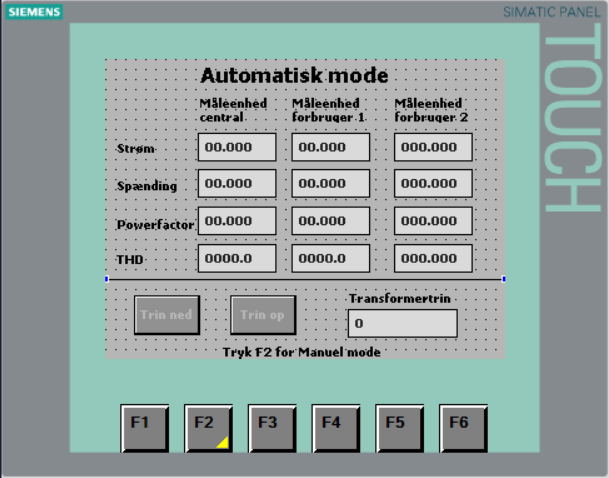
\includegraphics[width=0.7\textwidth]{Figure/HMIAutomatiskModeDesign}
	\caption{HMI i automatisk mode}
	\label{fig:HMIAutomatiskModeDesign}
\end{figure}

På begge skærme vises data for Måleenhederne i kolonner og rækker, for at give overblik. En mangel her er at det ikke er vist hvilken enhed, dataet vises i. For spænding er det i volt, strøm i ampere, power factor er enhedsløs og THD er vises som det samlede indhold af frekvenser i procent af den fundamentale frekvens. THD er forklaret i afsnit \ref{sec:THD}.


Under skillelinjen ses al information omkring Trinskifteren. I automatisk mode er det ikke muligt at skifte trin på knapperne Trin ned og Trin op, derfor er de gråskalerede. I manuel mode er de sort/hvid for at vise at de kan benyttes.


Knappen til tilstandsskift er på hver skærm placeret på F-knapperne med tilhørende forklarende tekst på skærmen, for at tydeliggør funktonaliteten af knapperne.


Systemet er klargjort til at en central og to decentrale Måleenheder, men i det endelige produkt er kun en central og en decentral Måleenhed. Forbruger 2 er derfor ikke aktiv i produktet.
% !TEX root = ../../prj4projektrapport.tex
% SKAL STÅ I TOPPEN AF ALLE FILER FOR AT MASTER-filen KOMPILERES 

\section{Kommunikationsmodul}

I starten af projektet var det tænkt at et separat kommunikationsmodul ikke var nødvendigt, da PSoC'en med et tilhørende Ethernetmodul ENC28J60 burde 

Kommunikationsmodulet består af en Arduino Mega2560 forbundet til et Ethernet Shield R3. Kommunikationsmodulet står for kommunikationen mellem Måleenhederne og Kontrolmodulet, det skal dermed modtage data fra Måleenhederne over UART kommunikation og sende det videre til Kontrolmodulet ved brug af TCP kommunikation. 

Arduinoen opsætter Ethernet Shield'et ved brug af en SPI forbindelse, der oprettes af SPI.h biblioteket, der kaldes som det første i koden. Dernæst er Ethernet.h biblioteket kaldt, for at kunne benytte de meget brugbare funktioner i dette bibliotek. 
% !TEX root = ../../prj4projektrapport.tex
% SKAL STÅ I TOPPEN AF ALLE FILER FOR AT MASTER-filen KOMPILERES 

\section{Test}

I dette afsnit vil der ikke blive gået i dybden med de enkelte tests, men derimod selve testprocessen og tankerne gjort i testfasen. For at se mere om de enkelte udførte test, se dokumentationen\footnote{Projektdokumentation, 10.4, Modultest}.

Da Styringsenheden generelt har indeholdt meget programmering, har det været oplagt at teste funktionaliteten af koden på nogel enheder på andre allerede udviklede og testede moduler i projektet.  Eksempelvis er funktionaliteten af Brugergrænsefladen testet med brug af andre allerede testede moduler. Til testen af Brugergrænsefladen er kommunikationen fra Måleenhed til Kommunikationsmodul og videre til Kontrolmodulet brugt for at genere tilfældige data, der så blev sendt til og udskrevet på HMI'en fra Kontrolmodulet. Det samme gælder testen af Arduinoens TCP modtagefunktion. Her er PLC'en benyttet  med et testprogram, der kan sende 'req1' kommandoen. Da man allerede har testet PLC'ens forbindelse på et andet Winsock testprogram, kan testen fokusere på Arduinoen. Herunder ses et enkelt testeksempel, hvor dette test program har været benyttet, se figur \ref{fig:EthernetTest}. For hele testbeskrivelsen refereres til dokumentationen\footnote{Projektdokumentation, 10.4.1, Kontrolmodul}.


\begin{figure}[H] % (alternativt [H])
	\centering
	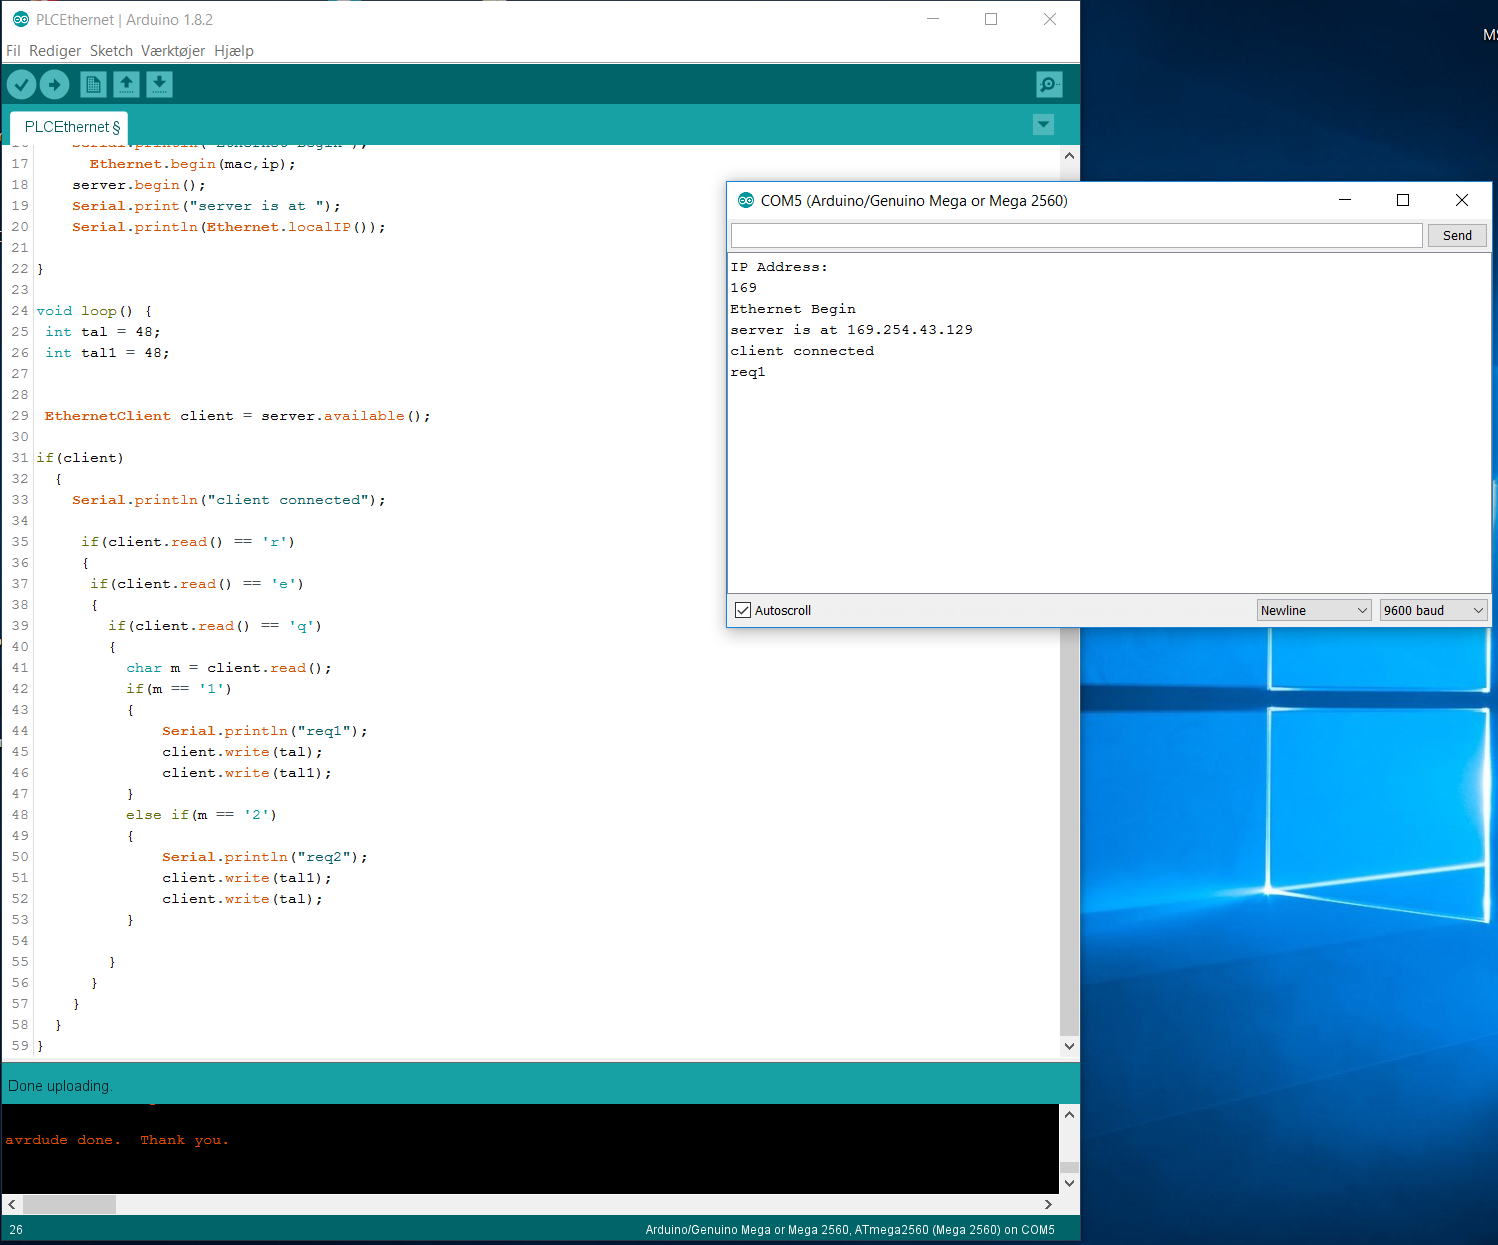
\includegraphics[width=0.85\textwidth]{figure/EthernetTest}
	\caption{Test af Arduinoens TCP data modtagelse}
	\label{fig:EthernetTest}
\end{figure}


% !TEX root =../prj4projektrapport.tex


\section{Delkonklusion}

I kapitel 5 er overvejelser omkring udvikling, design og implementering af Distributionslinje, Belastning og Trinskifter blevet beskrevet. Der er implementeret en simulering af en 60 km lang distributionslinje med modstand- og spolevirkning, der påvirker spændingsfald og power factor i systemet. Ligeledes er der implementeret belastninger, der kan til- og frakobles for at variere spændingsfaldet over disse. Endeligt er der implementeret en trinskifter i form af en trintransformer og et relækredsløb til skift af trin. På baggrund af modultest kan det konkluderes, at disse enheder giver mulighed for at lave det ønskede proof of concept.


\chapter{Resultat og Diskussion}
% !TEX root = ../prj4projektrapport.tex
% SKAL STÅ I TOPPEN AF ALLE FILER FOR AT MASTER-filen KOMPILERES 

I dette kapitel resultaterne for produktet af Spændingsregulator holdes op imod udformet kravspecifikation. Resultaterne vil blive diskuteret i forhold til, hvorledes kravene er opfyldt, og om løsningen er optimal. I kravspecifikationen er kravene delt op i funktionelle og ikke funktionelle krav. Det er lykkedes at opfylde alle kravene stillet i de funktionelle krav, hvorimod der er enkelte krav i de ikke funktionelle, som ikke er opfyldt. 

Det overordnede formål med udviklingen af prototypen for systemet er at bevise funktionaliteten og anvendeligheden af Spændingsregulatoren. Dette er fuldt ud lykkedes. Simuleringen af distributionslinjen er udviklet således, at Spændingsregulatorens evne til at overvåge og regulere spændingen i systemet tydeligt kommer til udtryk. Måleenheden er i stand til at måle spændingen ude ved forbrugeren, og sende de målte data til Styringsenheden. Reguleringen af spændingen foretages på baggrund af de målte data og kravet om $\pm10\%$ af 4V ved forbrugerne. Det er hermed bevist at Spændingsregulatoren er i stand til at holde spændingen stabil i et system ved varierende belastninger. 

Kommunikationen mellem Målenheden og Styringsenheden krævede at der blev udviklet et modul, som kan kommunikere med en Siemens PLC. Dette modul er essentielt for at Spændingsregulatoren fungerer som helhed. Anvendelsen af TCP-protokollen gjorde det muligt at udveksle data mellem modulet og PLC'en. 



% !TEX root = ../prj4projektrapport.tex
% SKAL STÅ I TOPPEN AF ALLE FILER FOR AT MASTER-filen KOMPILERES 

Den automatisk udviklede regulering er lavet ud fra en meget simpel model, hvor der skiftes lige så snart spændingen når et bestemt niveau. Det kunne være lavet bedre med hystereser, som gjorde at spændingen skulle være ved et bestemt niveau i noget tid, inden den skiftede. Det ville kunne give et mere stabilt system, da Spændingsregulatoren ville stå og skifte op og ned ved små ændringer omkring skiftene. Det er dog ikke noget problem i projektets simulerede belastninger da de springer i lidt større trin og ikke variere hele tiden.

Forbrugerne er dimensioneret efter at kunne lave en maks. strøm i systemet på 500mA, dette har dog vist sig ikke at kunne lade sig gøre, da Spændingsregulatoren ikke kan opretholde 4V ved forbrugerne, hvis de alle bliver slået til. Det er dog ikke prioriteret at gøre noget ved, da det har synes at være irrelevant. Det ville kunne have været løst ved at inddrage flere trin på transformeren.

Der er blevet lavet en prototype, der med stor tilfredshed har kunne simulere en løsning på problemformuleringen. I forhold til accepttesten\footnote{Projektdokumentation, 12, Accepttest}, har Spændingsregulatoren bevist at der kan skiftes trin på transformeren manuelt eller automatisk iht. hvor stor belastning der er i systemet. Derudover har den vist sig at kunne måle strøm og spænding i det simulerede systemet med høj præcision.
\chapter{Metode og proces}
% !TEX root = ../prj4projektrapport.tex
% SKAL STÅ I TOPPEN AF ALLE FILER FOR AT MASTER-filen KOMPILERES 

Til gennemførelse af dette projekt er ASE-modellen blevet anvendt som udgangspunkt. Denne model viser de forskellige faser, projektgruppen skal igennem på vejen mod et endeligt produkt og en veldokumenteret og gennemarbejdet rapport. ASE-modellen ses på figur \ref{fig:Asemodel} Gruppen har desuden anvendt en iterativ og empirisk arbejdsmetode. Der er brugt faglitteratur og teori fra undervisningen til at danne vidensgrundlag for projektet om spændingsregulatoren. Undervejs er der indsamlet nye erfaringer i forbindelse med udviklingen af produktet. 
I udviklingsfasen er der anvendt SysML og UML, der sammen med Use Casene har givet overblik over systemet både grafisk og skriftligt. Dette har dannet grundlag for opbygningen af systemet. 

\begin{figure}[H] 
	\centering
	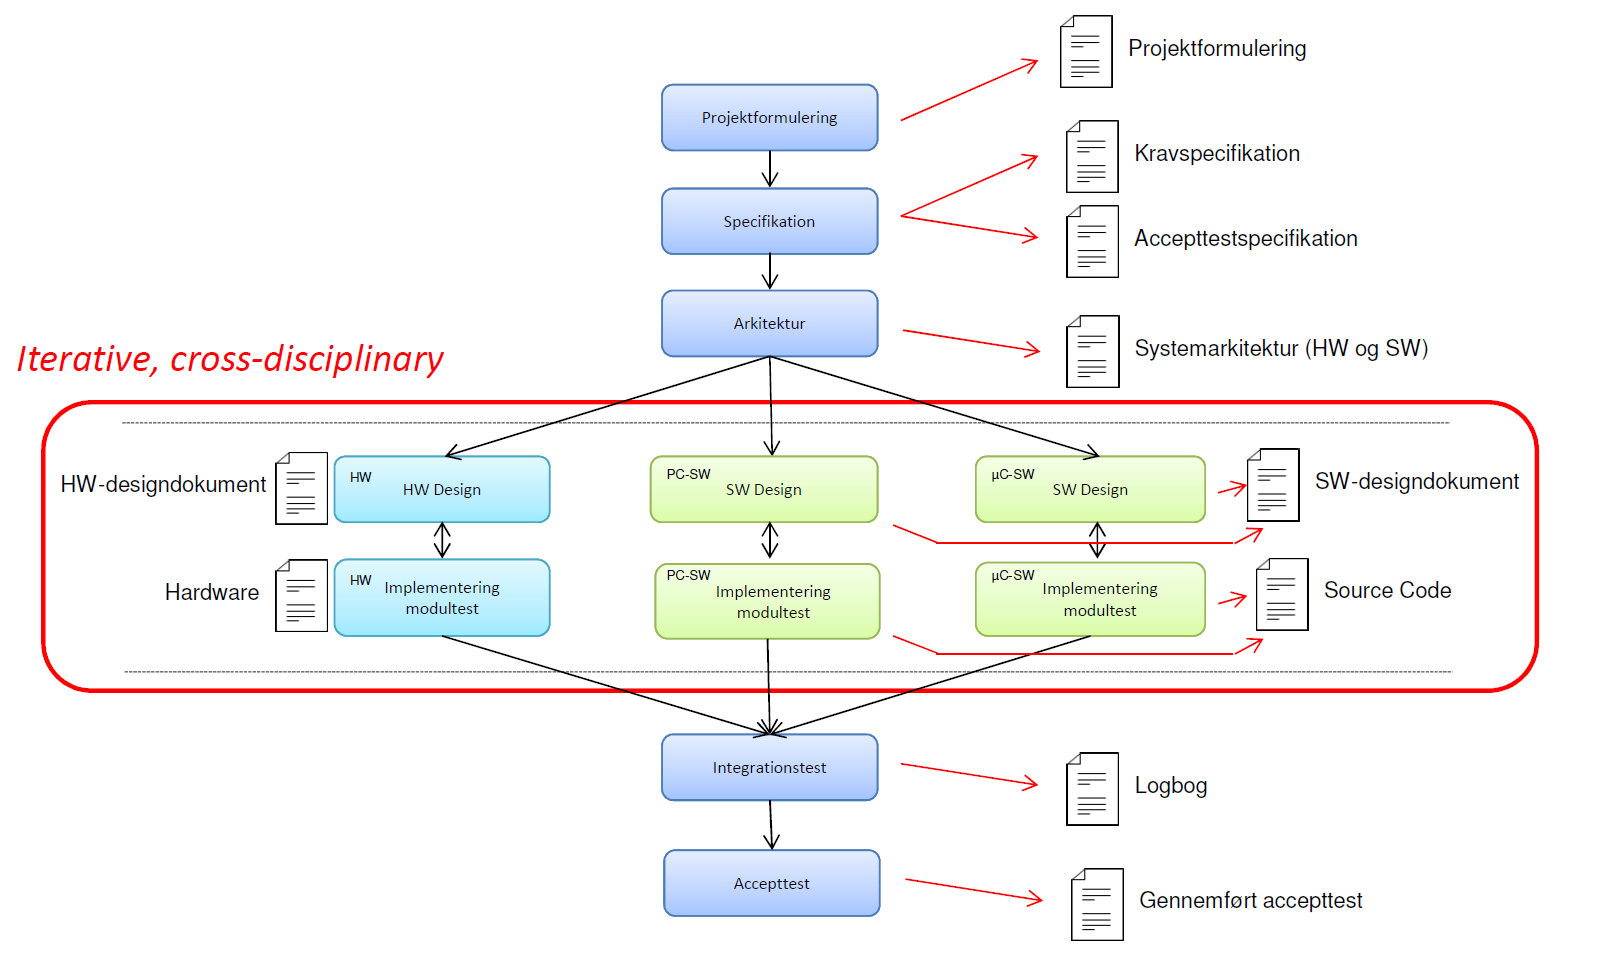
\includegraphics[width=0.7\textwidth]{figure/Asemodel}
	\caption{ASE-modellen}
	\label{fig:Asemodel}
\end{figure}

For at styre og lede projektet har gruppen ladet sig inspirere af Scrum principperne. Fra starten af projektet har gruppen oprettet sprints og defineret dertilhørende opgaver. Gruppen har ikke afholdt daily scrums, men har gennemsnitligt haft 1-2 ugentlige gruppemøder samt ugentligt vejledermøde. Gruppen udarbejdede desuden en tidsplan for udvikling og rapportskrivning, se bilag C5. Dette har medført en jævn arbejdsgang og et godt flow i projektet. \newline

Efter udfærdigelsen af arkitekturen for Spændingsregulatoren afholdt gruppen review med en anden projektgruppe. Efter rettelser herfra blev gruppen inddelt i tre hold med hvert sit ansvarsområde. Gennem design og implementeringsfasen har hvert hold haft ansvar for eget arbejdsområde, men den resterede del af gruppen er løbende blevet opdateret i forhold til udfordringer og løsninger. 
Ved integrationstest og accepttest er gruppen igen samlet, og disse udføres i fællesskab. 
Holdinddelingen og ansvarsområder ses i Tabel \ref{tab:arbejdsfordeling}.

% Please add the following required packages to your document preamble:
% \usepackage{booktabs}
% \usepackage{multirow}
\begin{table}[H]
	\centering
	\caption{Arbejdsfordeling}
	\label{tab:arbejdsfordeling}
	\begin{tabular}{@{}ll@{}}
		\toprule
		Navn                    & Arbejdsområde                                                  \\ \midrule
		Jeppe Hansen            & \multirow{2}{*}{Måleenhed}                                     \\
		Søren Jensen            &                                                                \\\midrule
		Laurids Givskov Jørgensen       & \multirow{2}{*}{Styringsenhed}                                 \\
		Dennis Slot Larsen            &                                                                \\\midrule
		Caroline Møller Sørensen       & \multirow{2}{*}{Distributionslinje, belastning og trinskifter} \\
		Sophia Amalie Mortensen &                                                                \\ \midrule
	\end{tabular}
\end{table}


\chapter{Fremtidigt arbejde}
% !TEX root = ../../prj4projektdokumentation.tex

\chapter{Design}

\section{Distributionslinje}
På baggrund af foranalysen er længden af distributionslinjen, der ønskes simuleret, valgt til 60 km. Ud fra datablade for den valgte kabeltype ses at der er vil være 0,1 $\omega$ /km og 0,219 mH/km. For at kunne simulere disse værdier er opbygget et kredsløb med 6,2 $\omega$ modstand i serie med en 13,6 mH spole. 




% !TEX root = ../../prj4projektrapport.tex
% SKAL STÅ I TOPPEN AF ALLE FILER FOR AT MASTER-filen KOMPILERES 

Måleenheden virker til det projekt og dermed den prototype der her er udviklet. Men i et endeleligt produkt ville det være optimalt at hardwaren blev ændret således der blev benyttet en instrumentationsforstærker i stedet for en enkelt OPAMP, således Måleenhed kunne måle differentielt og ikke skulle have et fikseret nulpunkt. 
% !TEX root = ../../prj4projektdokumentation.tex

\chapter{Design af Styringsenhed}

Styringsenheden er den del der skal sørge for at modtage data fra Måleenhederne og ud fra disse data styre trinskifteren. Til at koordinere kommunikation fra flere Målenheder til et Kontrolmodul er brugt en Arduino. Samtidig skal den informere en bruger om systemets tilstand gennem en burgergrænseflade. Her er anvendt en HMI. Kontrolmodulet er lavet på en PLC, der står for at opdatere trinskifteren og HMI ud fra de modtagede data.


\chapter{Perspektivering}
\chapter{Konklusion}

\printbibliography

\end{document}


